\documentclass[preprint,amsmath,amssymb,aps,pre]{revtex4-1}
% Latex
\usepackage[english]{babel}
\usepackage[utf8]{inputenc}
\usepackage[T1]{fontenc}
% Xelatex
%\usepackage{polyglossia}
%\usepackage{fontspec}
%\setdefaultlanguage{english}
%\setmainfont{DejaVu Sans}
%\setsansfont{DejaVu Sans}
%\setmonofont{DejaVu Sans Mono}
\usepackage{bm}
\usepackage{cleveref}
\usepackage{graphicx}
\usepackage{xcolor}
\usepackage{subfigure}

\definecolor{light-gray}{gray}{0.95}
\newcommand{\code}[1]{\colorbox{light-gray}{\texttt{#1}}}

% When cleveref fails to do its job
%\newcommand{\apref}[1]{Appendix \ref{#1}}

\begin{document}
%*Corresponding author: Kirill M. Gerke, Tel.: +79661877715, E-mail: kg@ifz.ru,
%Address: Schmidt Institute of Physics of the Earth of Russian Academy of
%Sciences, Bolshaya Gruzinskaya str. 10/1, Moscow, 123242, Russia
\author{Vasily Postnicov}
\affiliation{Schmidt Institute of Physics of the Earth of Russian Academy of
  Sciences, Moscow, 123242, Russia}
\author{Alexey I. Samarin}
\altaffiliation{Computational Mathematics and Cybernetics, Lomonosov Moscow
  State University, Moscow, 119991, Russia}
\affiliation{Schmidt Institute of Physics of the Earth of Russian Academy of
  Sciences, Moscow, 123242, Russia}
\author{Efim V. Lavrukhin}
\altaffiliation{Computational Mathematics and Cybernetics, Lomonosov Moscow
  State University, Moscow, 119991, Russia}
\affiliation{Schmidt Institute of Physics of the Earth of Russian Academy of
  Sciences, Moscow, 123242, Russia}
\author{Marina V. Karsanina}
\affiliation{Schmidt Institute of Physics of the Earth of Russian Academy of
  Sciences, Moscow, 123242, Russia}
\author{Mathieu Gravey}
\altaffiliation{University of Lausanne, Faculty of Geosciences and Environment,
  Institute of Earth Surface Dynamics, Lausanne, Switzerland}
\author{Kirill M. Gerke}
\email[E-mail:]{kg@ifz.ru}
\affiliation{Schmidt Institute of Physics of the Earth of Russian Academy of
  Sciences, Moscow, 123242, Russia}

\title{Cool simulated annealing package}

\begin{abstract}
  What have we done?
\end{abstract}

\maketitle

\section{Overview of simulated annealing algorithm}
\label{sec:annealing}
The goal of our work is to create a two or three dimensional binary image $A$
which minimizes some non-negative target function $f(A, B)$. This function
usually includes difference in correlation functions, such as two-point or
lineal-path correlation function, between the image $A$ and the target (or
original) image $B$. The image $B$ is not necessarily known but can instead be
described by a set of correlation functions. The algorithm which minimizes the
target function is an iterative algorithm called \textit{simulated
  annealing}. The principle of work is following:
\begin{enumerate}
\item Take $A$ as an inititial approximation of $B$.
\item Let $T_0$ be a real-valued parameter called \textit{temperature}.
\item Let $f_1 = f(A, B)$
\item Let $S$ be any number of samples taken from $A$ (indices into $A$) using
  a sample function $s(A)$.
\item Modify samples $S$ using a modification function $m$ and assign the result
  to $S'$: $S' = m(S)$. Create a new image $A'$ by replacing samples $S$ with
  $S'$.
\item Let $f_2 = f(A', B)$.
\item For k-th iteration of the simulated annealing replace $A$ with $A'$ with
  probability
  \begin{equation*}
    p =
    \begin{cases}
      1 & \text{if } f_2 < f_1 \\
      \exp(-\frac{f_2 - f_1}{T_k}) & \text{otherwise}
    \end{cases}
  \end{equation*}
  otherwise just discard $A'$.
\item Assign a new value $c(T_k, f_2)$ to $T_{k+1}$.
\item Repeat from the third step until some requirements are met, e.g.
  $f(A, B) < \epsilon$.
\end{enumerate}
This algorithm requires a selection of five parameters: a value $T_0$, a target
function $f(A, B)$, a sampler function $s(A)$, a modifier function $m(S)$ and a
function $c(T, f)$, called \textit{cooldown schedule}. Also we need to define a
way in which an initial approximation is obtained. This results in six
configurable options which can be tuned in order to obtain the best result. A
process of generating an initial approximation is discussed in section
\cref{sec:init}, possible target functions are discussed in \cref{sec:target},
sampler and modifier functions are discussed in \cref{sec:samplers-mods} and
cooldown schedules are discussed in \cref{sec:cooldown}.

\section{Initial approximations}
\label{sec:init}
In this section we discuss how initial images for the first part of simulated
annealing algorithm can be created.
\subsection{Using uniformly distributed noise}
\label{sec:init-uniform}
\textbf{FIXME: Is this noise really ``uniformly distributed''?}
To approximate a binary image $B$ we create an image $A$ consisting entirely of
void phase. Then we change a randomly selected sample in $A$ to be in solid
phase. The sample is taken according to a uniform distribution. We then repeat
this process, independently taking and changing another sample until porosity of
the image $A$ equals to porosity of the image $B$. In this case we start the
algorithm with $S_2(A, 0) = S_2(B, 0) = L_2(A, 0) = L_2(B, 0)$ where $S_2$ is
the two-point correlation function and $L_2$ is the lineal-path correlation
function.
\subsection{Using overlapped balls}
\label{sec:init-balls}
As described in \cite{torq-book}, analytic representation of $S_2$ and $L_2$
functions is well known for overlapping balls of radius $R$ with centers
generated by Poisson point process with a parameter $\lambda$. An expression for
$S_2$ function is following:
\begin{equation}
  S_2(r, R, \lambda) = \exp(-\lambda v_1(R) v_2(r, R)) \label{eq:s2-balls}
\end{equation}
where $v_1(R)$ is a volume of n-dimensional ball and
\begin{equation*}
  v_2(r, R) =
  \begin{cases}
    2H(r - 2R) + \frac{2}{\pi}[\pi + \frac{r}{2R}(1 - \frac{r^2}{4R^2})^{1/2} -
      \arccos(\frac{r}{2R})]H(2R-r) & n = 2 \\
    2H(r - 2R) + [1 + \frac{3}{4}\frac{r}{R} - \frac{1}{16}(\frac{r}{R})^3]H(2R
    - r) & n = 3
  \end{cases}
\end{equation*}
where $H(x)$ is Heaviside step-function.

The method of making an initial approximation is as follows:
\begin{enumerate}
\item Calculate two-point correlation function $S_2(B)$ of the original image
  $B$.
\item Find parameters $R, \lambda$ so that \cref{eq:s2-balls} fits
  $S_2(B)$. This can be done using well-known least-squares method.
\item Generate a set of centers $C$ using a realization of Poisson point process
  with parameter $\lambda$.
\item Draw balls of radius $R$ with centers in $C$.
\end{enumerate}
This method results in faster convergence of simulated annealing algorithm when
the target function takes $S_2$ into account. For good results it is neccessary
for number of generated centers to be big enough. Note that for this method
$S_2(A, 0) \ne S_2(B, 0)$ and $L_2(A, 0) \ne L_2(B, 0)$.
\begin{figure}[ht]
  \centering
  \subfigure[Target image]{
    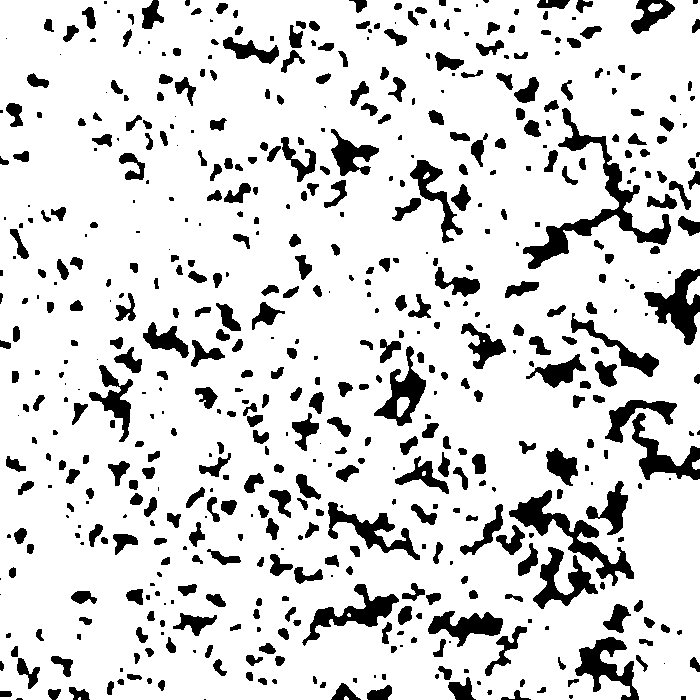
\includegraphics[width=0.45\linewidth]{../images/balls-orig.png}
    \label{fig:init-balls-target}}
  \hfill
  \subfigure[Initial approximation]{
    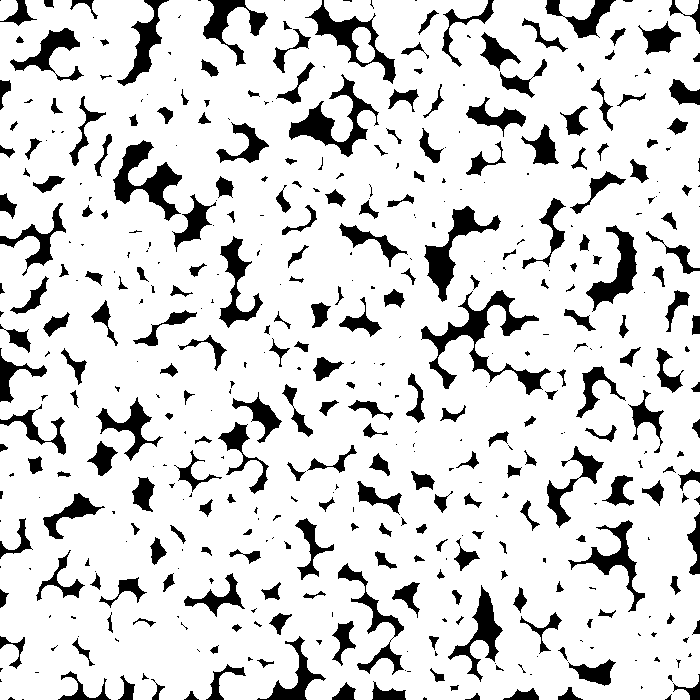
\includegraphics[width=0.45\linewidth]{../images/balls-init.png}
    \label{fig:init-balls-init}}
  \caption[]{An example of a target image and an initial approximation by
    overlapping balls.}
  \label{fig:init-balls}
\end{figure}

\begin{figure}[ht]
  \centering
  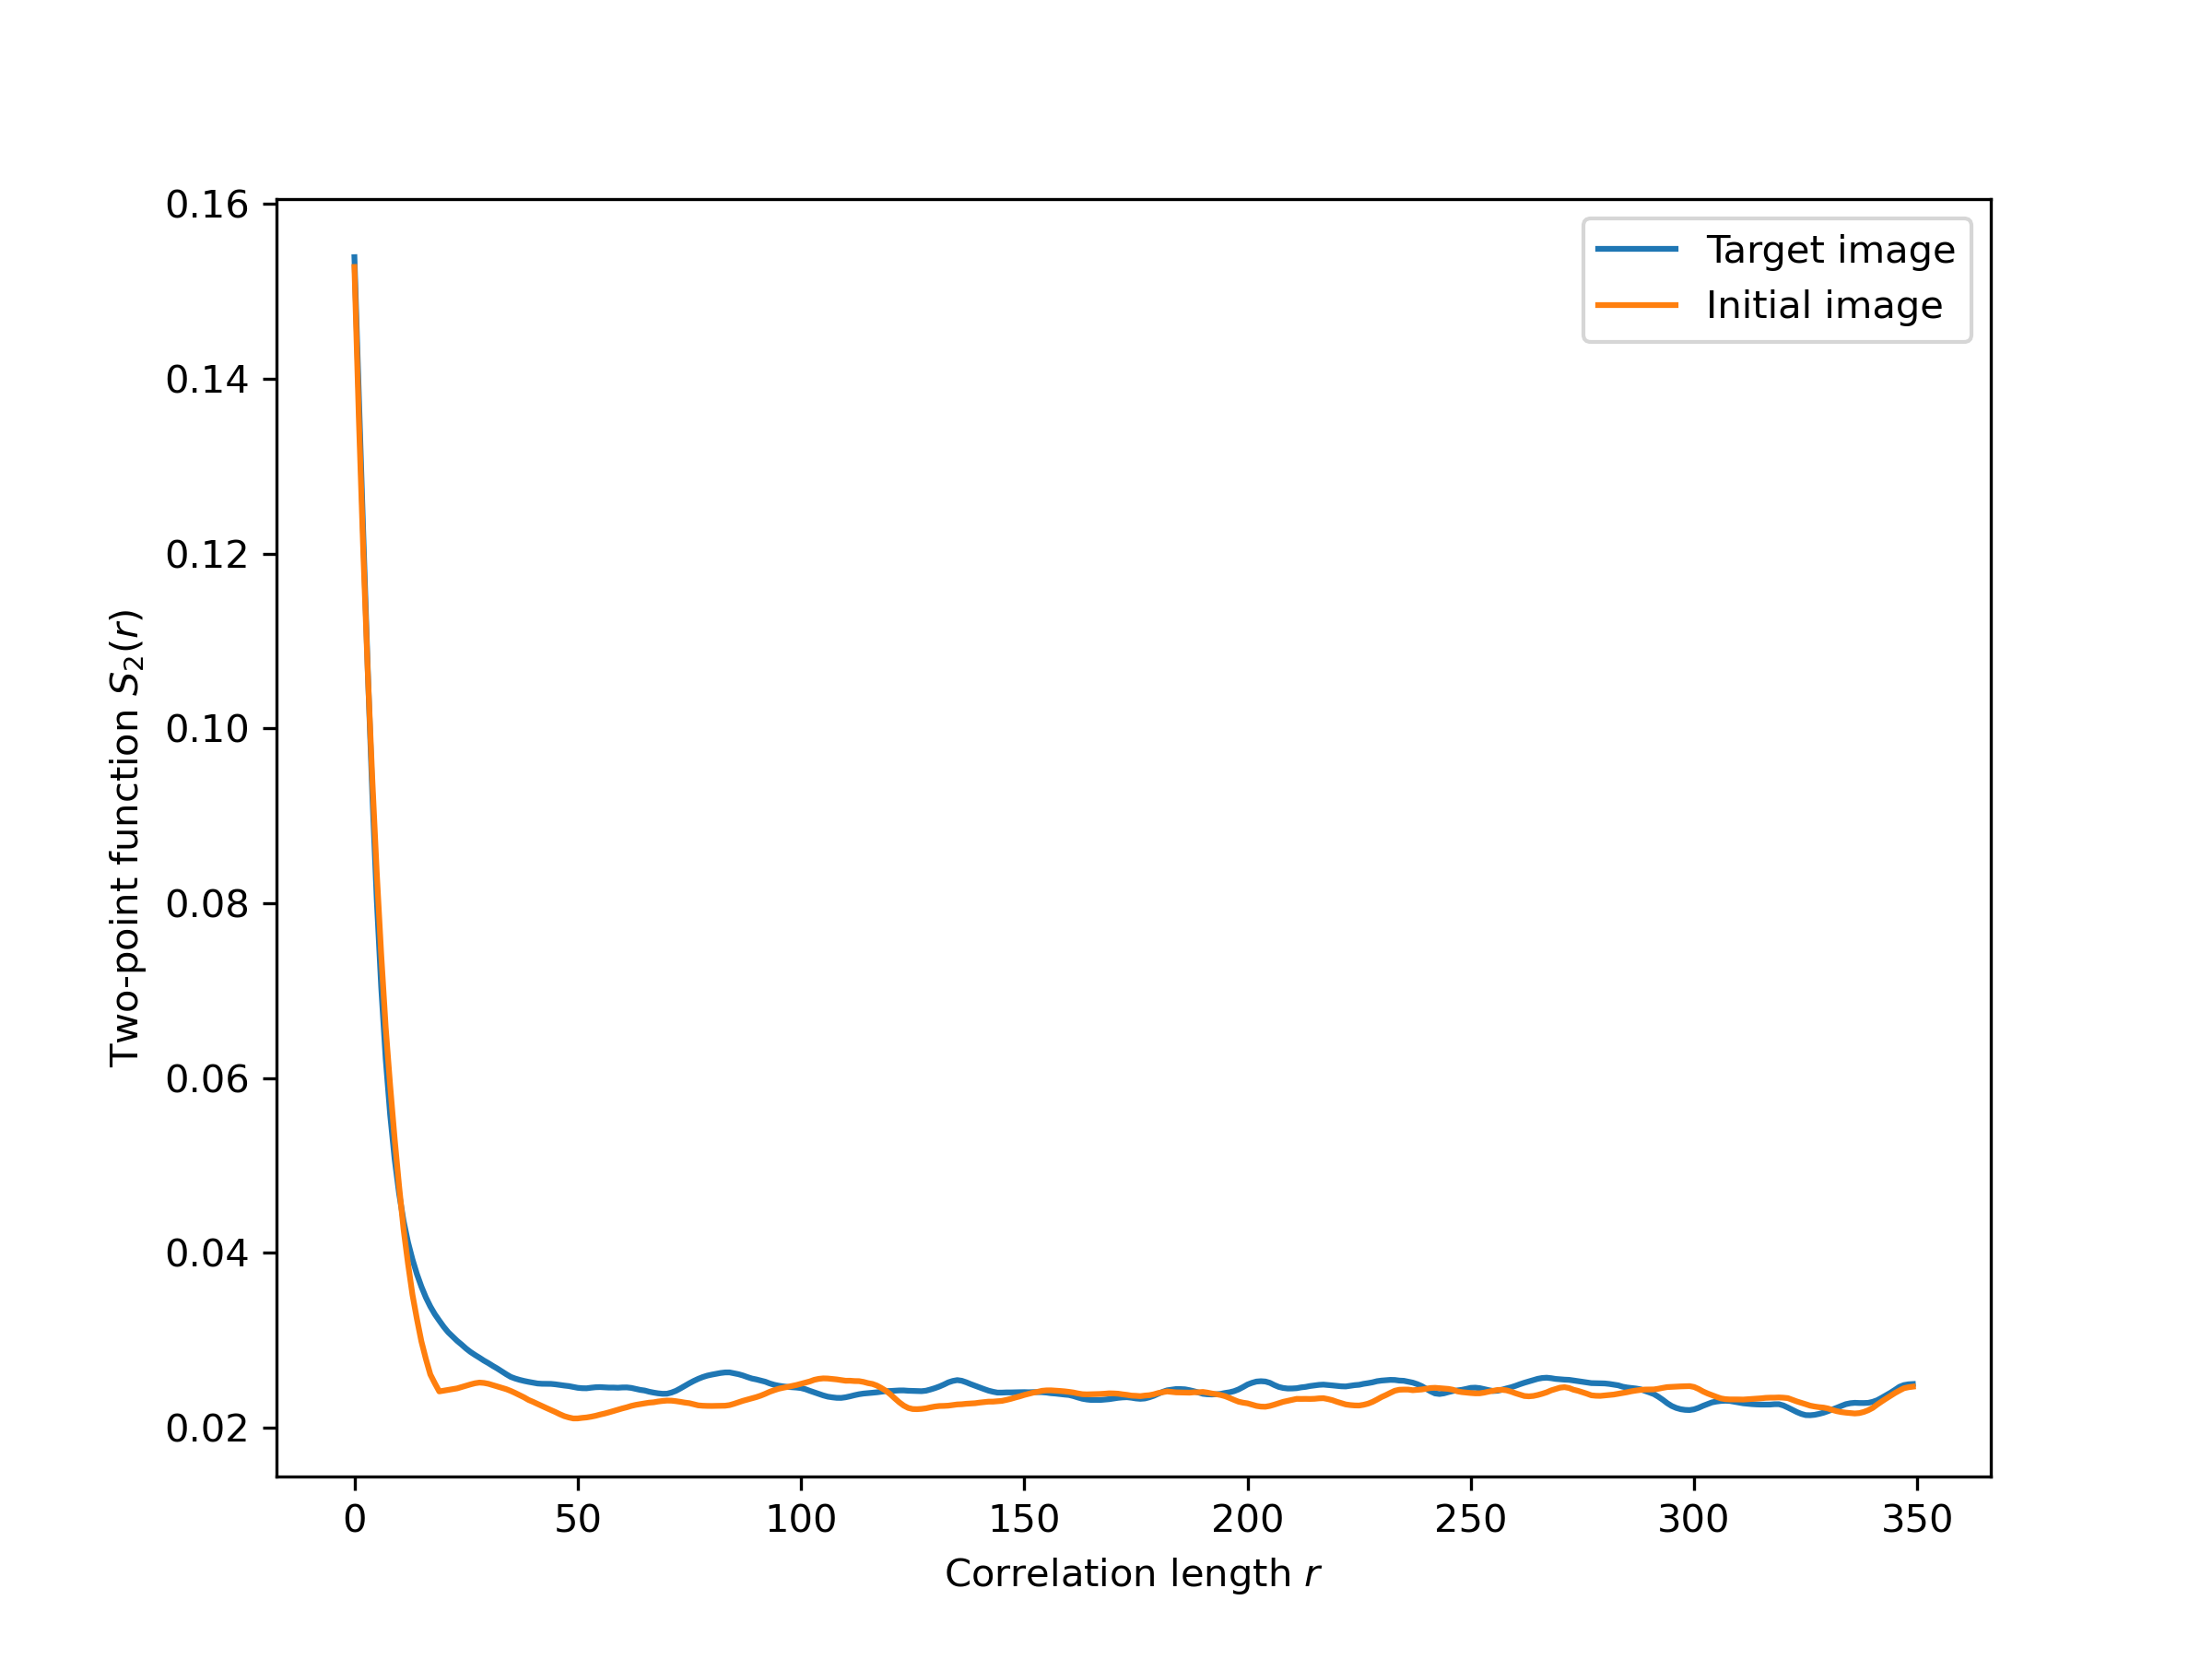
\includegraphics[width=\linewidth]{../corrfns-plots/init-s2.png}
  \caption[]{Two-point correlation function for the target image and the initial
  approximation show on \cref{fig:init-balls}.}
  \label{fig:init-balls-s2}
\end{figure}

\section{Target functions}
\label{sec:target}
In this section we discuss target functions used in our package. At first we
define difference between images $A$ and $B$ measured with respect to
correlation function $cf$ as
\begin{equation*}
  \Delta_{cf}(A, B) = \sum_{n=0}^{N} \sum_{i} (F_c(A, n\mathbf{x}_i) - F_c(B, n\mathbf{x}_i))^2
\end{equation*}
Here $n$ is a correlation length and $\mathbf{x}_i$ is a direction at which
correlation function is calculated. We can calculate correlation functions along
axial directions (e.g. $(1,0,0)$, $(0, 1, 0)$ and $(0, 0, 1)$ for 3D images) and
diagonal directions which results in total of 4 directions for 2D images and 13
directions for 3D images.

At each step of simulated annealing algorithm we can fastly update $S_2$ and
$L_2$ functions and also $F_{ss}$ (surface-surface) and $F_{sv}$ (surface-void)
functions, so these four functions are usually taken into account.

\subsection{Weighted target function}
\label{sec:target-weighted}
Weighted target function \cite{gerke-target} defined as
\begin{equation*}
  f_w(A, B) = \sum_{n=1}^{N} \frac{\Delta_{f_n}(A, B)}{\Delta_{{f_n}0}}
\end{equation*}
where $\Delta_{{f_n}0} = \Delta_{f_n}(A, B)$ before any modifications are made
to $A$. The initial value of $f_w(A, B)$ is $N$. Any number $N$ of correlation
functions may participate in this target function.

\subsection{Čapek target function}
\label{sec:target-čapek}
The original target function proposed by Čapek \cite{capek-target} is
\begin{align*}
  f_c(A, B) = e_1 & + e_2 + e_3 \frac{\eta}{\eta + e_1 + e_2} \\
  e_1 & = \Delta_{S^{(void)}_2}(A, B) \\
  e_2 & = \Delta_{L^{(solid)}_2}(A, B) \\
  e_3 & = \Delta_{L^{(void)}_2}(A, B)
\end{align*}
The parameter $\eta$ is usually set to $0.3-0.5$. In this function influence of
$L_2^{(void)}$ increases with decrease of the target function.

\subsection{Generalized Čapek target function}
\label{sec:target-čapek-general}
This target function is a generalization of the function described in
\cref{sec:target-čapek} for use with surface-surface and surface-void
functions. It is defined as
\begin{align*}
  f_{gc}(A, B) = e_1 + e_2 + e_3 \frac{\eta_1}{\eta_1 + e_1 + e_2} & + e_4
  \frac{\eta_2}{\eta_2 + e_1 + e_2} + e_5 \frac{\eta_2}{\eta_2 + e_1 + e_2} \\
  e_1(A, B) & = \Delta_{S^{(void)}_2}(A, B) \\
  e_2(A, B) & = \Delta_{L^{(solid)}_2}(A, B) \\
  e_3(A, B) & = \Delta_{L^{(void)}_2}(A, B) \\
  e_4(A, B) & = \Delta_{F^{(void)}_{ss}}(A, B) \\
  e_5(A, B) & = \Delta_{F^{(void)}_{sv}}(A, B)
\end{align*}
where $\eta_1$ and $\eta_2$ are two parameters in the range $0.3-0.5$.

\section{Samplers and modifiers}
\label{sec:samplers-mods}
In this section we discuss sampler functions $s(A)$ along with modifier
functions $m(S)$. A composed function $m \circ s$ is a function which modifies
the image $A$ and produces a new image $A'$ at each step of the simulated
annealing algorithm. 
\subsection{Uniform sampler}
\label{sec:sampler-uniform}
This sampler is the most simple one. It takes a sample according to a uniform
distribution. Usually, the use of this sampler results in very slow decrease of
the target function, so we use more advanced samplers like ones described in
\cref{sec:sampler-dpn} or \cref{sec:sampler-interface} whenever possible.

\subsection{Different phase neighbors-based sampler}
\label{sec:sampler-dpn}
Motivation behind this sampler is simple: we take a sample $s_c$ from an image
and look at its neighbors. If a number of neighbors which have a phase different
from a phase of $s_c$ is high when probably this sample is ``lost'' in a region
of alien phase and is subject for modification. The goal is to create regions of
(locally) the same phase and more ``smooth'' image.

A probability of taking any fixed sample $s_c$ with a uniform sampler described
in \cref{sec:sampler-uniform} is $P = \frac{1}{N}$ where $N$ is a total number
of pixels or voxels in the image. Now suppose that the set $S$ of all samples of
the image is divides into $n$ disjoints sets $S_i$:
\begin{align*}
  S &= \bigcup_{i=0}^{n-1} S_i \\
  S_i \cap S_j &= \varnothing \quad \text{for } \forall i,j: i \ne j
\end{align*}

Now suppose $A$ is an event of choosing any fixed sample $s_c$ and $B_i$ is an
event of choosing a sample from the set $S_i$. The probability of choosing the
sample $s_c$ equals to
\begin{equation*}
  P(A) = \sum_{i = 0}^{n-1} P(A|B_i) P(B_i) = \frac{1}{N}
\end{equation*}
where $P(B_i) = \frac{N_i}{N}$ and $P(A|B_i) = \frac{1}{N_i}$ if $s_c \in S_i$
and zero otherwise. $N_i$ is these equations means a number of samples in the
set $S_i$.

The sampling method described in \cref{sec:sampler-uniform} is equivalent to
these two steps:
\begin{enumerate}
\item Choose a set $S_i$ with probability $\frac{N_i}{N}$.
\item Uniformly choose a sample in this set.
\end{enumerate}
We can put an emphasis on sets with bigger value of $i$, so the probability of
choosing a set $S_i$ becomes
\begin{equation}
  P(B_i) = \alpha^i \beta \frac{N_i}{N} \quad \text{for } \alpha > 1 \label{eq:prob-dpn}
\end{equation}
where $\beta$ can be found from an equation
\begin{equation*}
  \beta (\sum_{i=0}^{n-1} \alpha^i \frac{N_i}{N}) = 1
\end{equation*}

The disjoint sets $S_i$ are chosen by analizing the number of different phase
neighbors for each voxel or pixel. A sample $x$ belongs to the set $S_i$ if a
set $\left\{ x_j: \rho(x, x_j) = 1 \land A(x_j) \ne A(x) \right\}$  contains $i$
elements. Here $\rho(x,y)$ denotes the Chebyshev distance. The sampling
algorithm consists of the previosly described two steps with the probability
$\frac{N_i}{N}$ replaced by \cref{eq:prob-dpn}.

\subsection{Sampling on the phase interface}
\label{sec:sampler-interface}
This sampler generates a random starting index $S_0$ in $A$ and a vector
$\delta: |\delta| = 1$. Then it finds minimal positive $n$ so that
$A(s_0) \ne A(s_0 + n\delta)$. An index $s_0 + \lfloor n\delta \rfloor$ is a new
sample. The point is that all samples generated this way belong to an interface
between phases.

\subsection{Flipper modifier}
\label{sec:flipper}
This modifier function is used to reconstruct binary images. Binary image is
an image which contains only elements $v$ and $s$ (\textit{void} or
\textit{solid} respectively). Flipper modifier takes one sample and ``flips''
the phase of that sample, changing $v$ to $s$ and vice-versa.

\subsection{Swapper modifier}
\label{sec:swapper}
The Swapper modifier function takes a pair of samples $(s_1, s_2)$ with
$A(s_1) \ne A(s_2)$ and ``swaps'' the phases of these samples
($A(s_1) \rightarrow A(s_2), A(s_2) \rightarrow A(s_1)$). This modifier function
preserves porosity of two-phase images, so it is unsuitable for use with
initialization algorithm described in \cref{sec:init-balls}.

\section{Cooldown schedules}
\label{sec:cooldown}
We use three well-known cooldown schedules, namely, exponential cooldown,
Aarts-Korst schedule \cite{Aarts-Korst} and Frost-Heinemann
\cite{Frost-Heinemann} schedule. All these schedules depend on two parameters:
$n \in \mathbb{N}$ and $\lambda \in \mathbb{R}$. In all the schedules $n$ is
choosen big enough to achieve thermodynamic equilibrium before the temperature
decreases. Thermodynamic equilibrium is a state when a number of accepted
changes is roughly equal to a number of rejected changes when the most recent
changes are taken into consideration. $\lambda$ must be in the range $0.85-0.95$
for the exponential cooldown and $0.001-1.0$ for other schedules.

\subsection{Exponential cooldown schedule}
\label{sec:cooldown-exp}
Exponential cooldown is the simplest cooldown schedule. For k-th step of the
simulated annealing a new value of temperature is calculated as
\begin{equation*}
  T_{k+1} =
  \begin{cases}
    T_k, & k \ne ln, l \in \mathbb{N} \\
    \lambda T_k, & \text{otherwise}
  \end{cases}
\end{equation*}

\subsection{Aarts-Korst cooldown schedule}
\label{sec:cooldown-aarts-korst}
In this schedule the temperature is updated on each n-th step as in
\cref{sec:cooldown-exp}, but this time instead of simply multiplying $T$ on
constant parameter $\lambda$ we define a new value of temperature as
\begin{equation*}
  \frac{1}{T_{l+1}} = \frac{1}{T_l} + \frac{\lambda}{\sigma_l}
\end{equation*}
where $l \in \mathbb{N}$ is a multiple of $n$ and $\sigma_{l}$ is standard
deviation of values of target function on steps $l-n, \dots, l$.

\subsection{Frost-Heinemann cooldown schedule}
\label{sec:cooldown-frost-heinemann}
As in two previous schedules the temperature updates every n-th step. Also there
is an auxiliary value $\hat{E}_l$ called \textit{target mean energy} which also
updates every n-th step. New values for temperature and target mean energy are
calculated as
\begin{align*}
  \hat{E}_{l+1} & = \overline{E}_l - \lambda \sigma_l \\
  T_{l+1} & = T_l + (\hat{E}_{l+1} - \hat{E}_l)\frac{T^2_l}{\sigma^2_l}
\end{align*}
where $\overline{E}_l$ is mean value of target function calculated for
steps $l-n,\dots,n$ and $\sigma_l$ is standard deviation of values of
target function for the same range of steps and $\hat{E}_0 = \overline{E}_0$.

\section{Results}
In this section we provide reconstructions of some two-dimensional images
including a checkerboard, randomly generated overlapping monodisperse disks,
rotated and thresholded value noise and a sandstone. The images are
reconstructed using two sets of correlation functions:
\begin{enumerate}
\item Two-point correlation function $S_2(r)$ and lineal-path correlation
  functions for solid $L_2^{(1)}(r)$ and void $L_2^{(0)}(r)$ phases.
\item Functions from the first set plus surface-surface correlation function
  $F_{ss}(r)$ and surface-void correlation function $F_{sv}(r)$.
\end{enumerate}
These correlation functions are calculated in two axial and two diagonal
directions.

All images are reconstructed using a cooldown schedule proposed by Aarts and
Korst \cite{Aarts-Korst} with parameters $n = 200$ and $\lambda = 0.007$ in 9
million iterations. For each reconstructed image we provide a plot of difference
between correlation functions of the original and reconstructed images as a
function of correlation length (averaged over all directions) as well as an
image showing difference between two-point correlation maps.

When the first set of correlation functions is chosen for a reconstruction, we
use a target function described in \cref{sec:target-čapek}, otherwise, a
function described in \cref{sec:target-čapek-general} is used. A modifier used
in all reconstruction is described in \cref{sec:flipper}.

\subsection{Checkerboard}
The original image has dimensions 500x500 pixels with dimensions of a single
square being 32x32 pixels. Uniformly distributed(?) noise was picked as an
initial approximation of the original. The sampler used in the reconstruction is
described in \cref{sec:sampler-dpn}. The original and reconstructed images can
be seen on \cref{fig:check-orig} -- \cref{fig:check-all}. The difference between
reconstructed and original correlation functions is on
\cref{fig:check-corr-s2l2} -- \cref{fig:check-corr-all}. As you can see,
addition of surface-surface or surface-void correlation functions to the target
function does not improve the result much in this particular case.

\subsection{Overlapping disks}
The original image of overlapping monodisperse disks has dimensions 500x500
pixels. All parameters are chosen to be the same as for the case with
checkerboard. The original and reconstructed images can be seen on
\cref{fig:disks-orig} -- \cref{fig:disks-all}. The difference between
reconstructed and original correlation functions is on
\cref{fig:disks-corr-s2l2} -- \cref{fig:disks-corr-all}.

\subsection{Value noise}
The original image has dimensions 1000x1000 pixels and was produced by
generating two dimensional value noise with \verb+ValueNoise.jl+ package,
thresholding and rotating it on $-\pi/4$ radians. A set of overlapping spheres
was used as an initial approximation of the original images, and the sampler
used in reconstruction procedure is described in \cref{sec:sampler-interface}.

\begin{figure*}[htp]
  \centering
  \subfigure[Checkerboard]{
    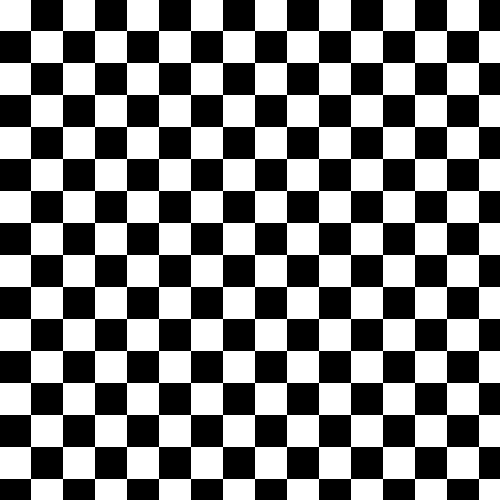
\includegraphics[width=0.3\textwidth]{../images/checkboard-orig.png}
    \label{fig:check-orig}}
  \hfill
  \subfigure[Reconstruction of \cref{fig:check-orig} using set 1]{
    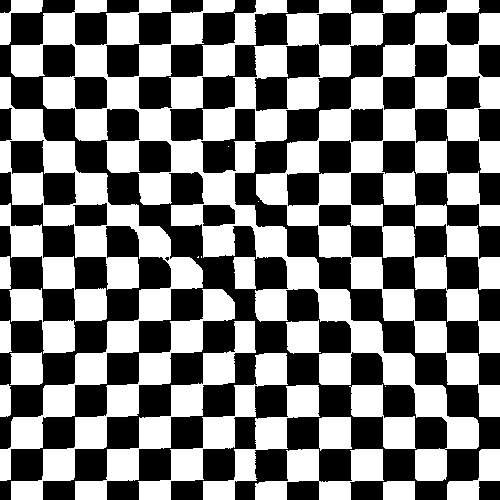
\includegraphics[width=0.3\textwidth]{../images/checkboard-s2l2.png}
    \label{fig:check-s2l2}}
  \hfill
  \subfigure[Reconstruction of \cref{fig:check-orig} using set 2]{
    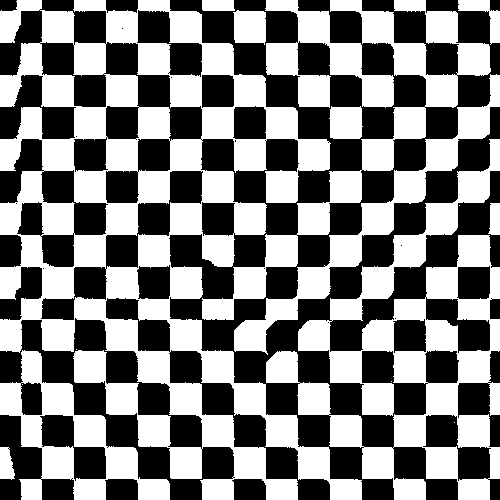
\includegraphics[width=0.3\textwidth]{../images/checkboard-all.png}
    \label{fig:check-all}}
  \vskip\baselineskip
  \subfigure[Small overlapping disks]{
    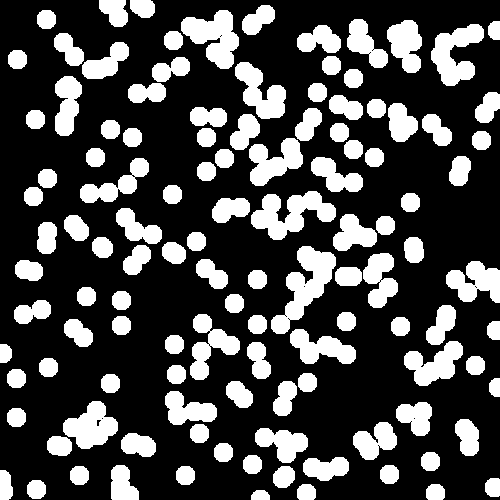
\includegraphics[width=0.3\textwidth]{../images/disks-orig.png}
    \label{fig:disks-orig}}
  \hfill
  \subfigure[Reconstruction of \cref{fig:disks-orig} using set 1]{
    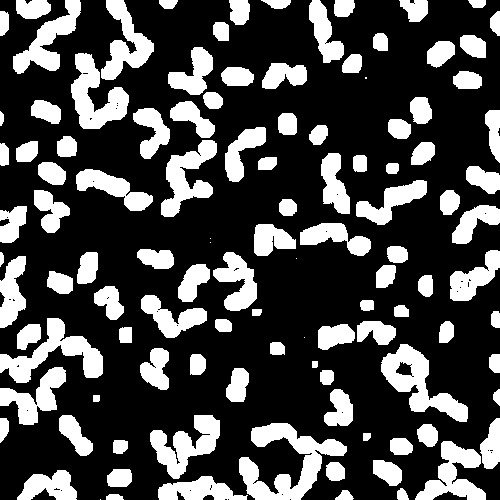
\includegraphics[width=0.3\textwidth]{../images/disks-s2l2.png}
    \label{fig:disks-s2l2}}
  \hfill
  \subfigure[Reconstruction of \cref{fig:disks-orig} using set 2]{
    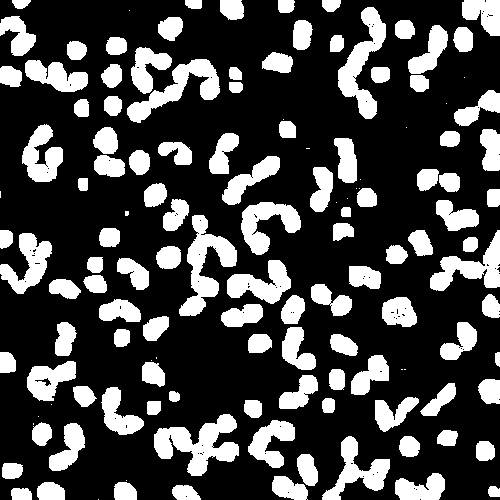
\includegraphics[width=0.3\textwidth]{../images/disks-all.png}
    \label{fig:disks-all}}
  \caption[]{Original images and their reconstructions}
  \label{fig:orig-recon1}
\end{figure*}

\begin{figure*}[htp]
  \centering
  \subfigure[Value noise]{
    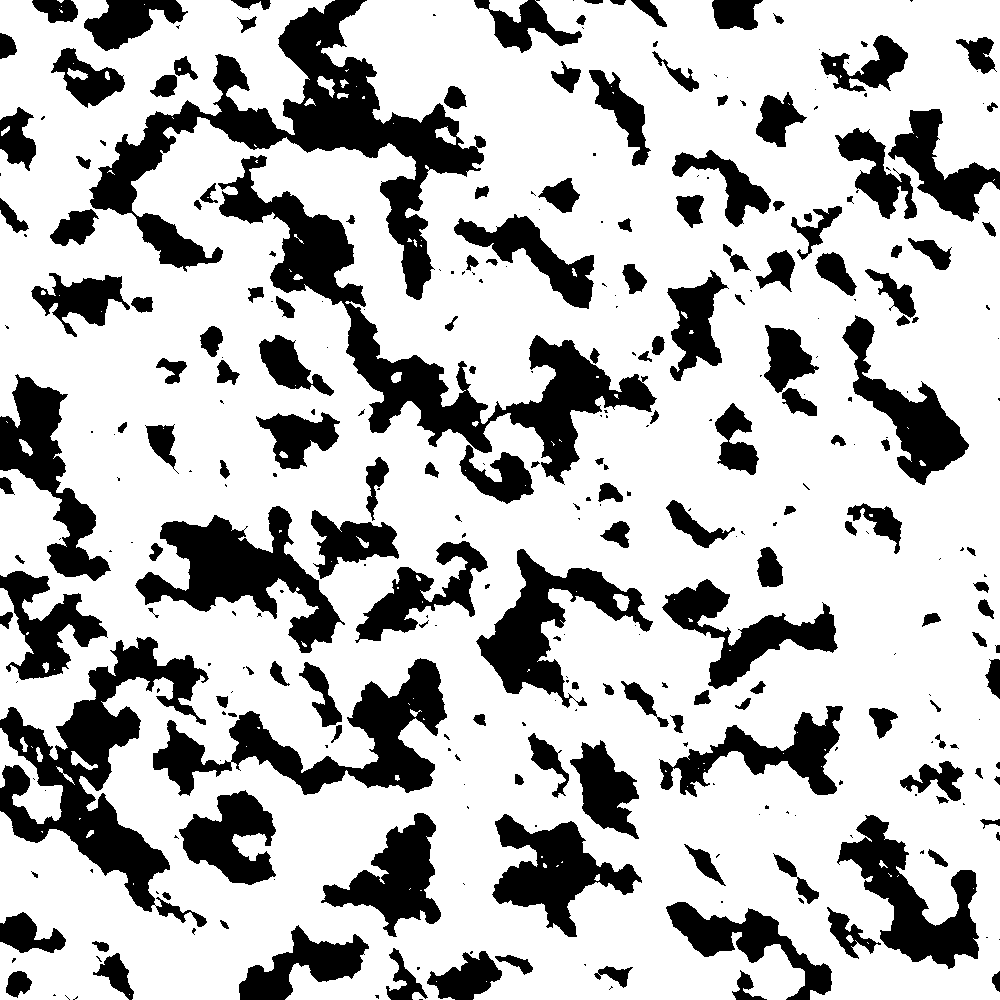
\includegraphics[width=0.3\textwidth]{../images/noise-orig.png}
    \label{fig:noise-orig}}
  \hfill
  \subfigure[Reconstruction of \cref{fig:noise-orig} using set 1]{
    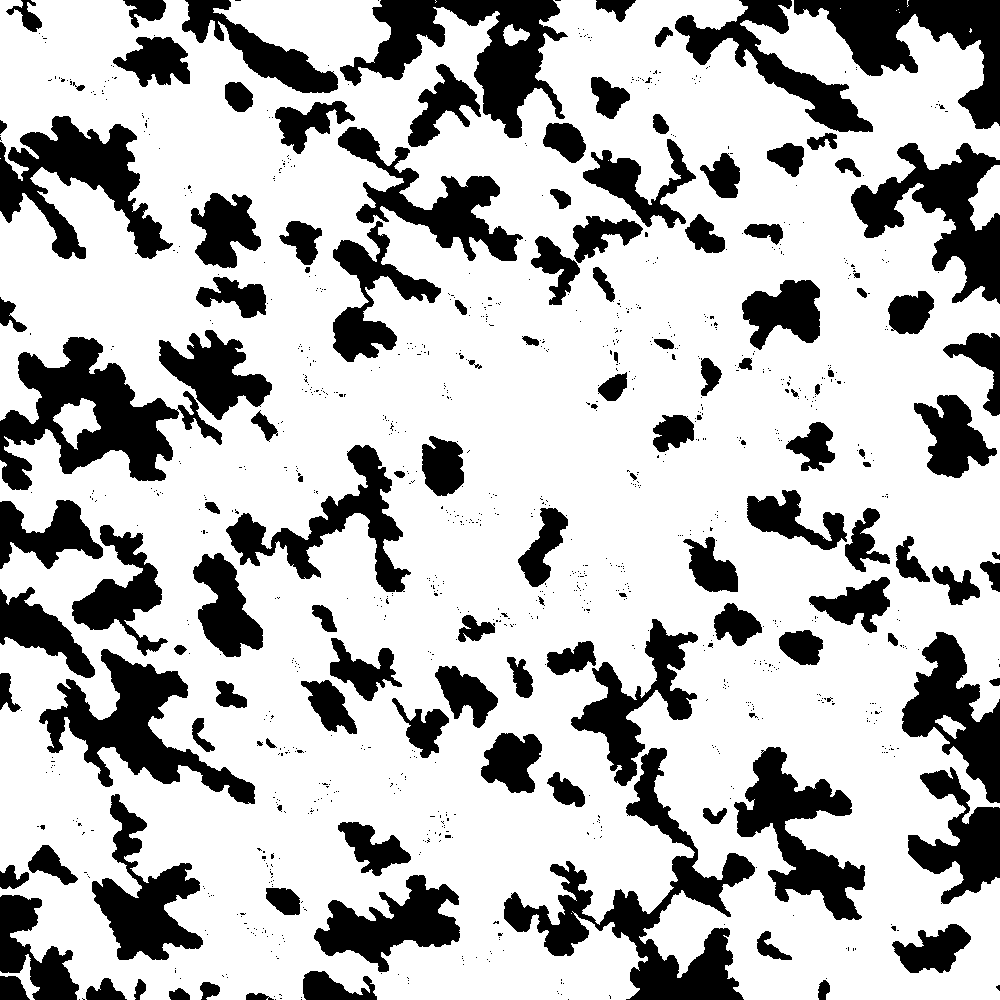
\includegraphics[width=0.3\textwidth]{../images/noise-s2l2.png}
    \label{fig:noise-s2l2}}
  \hfill
  \subfigure[Reconstruction of \cref{fig:noise-orig} using set 2]{
    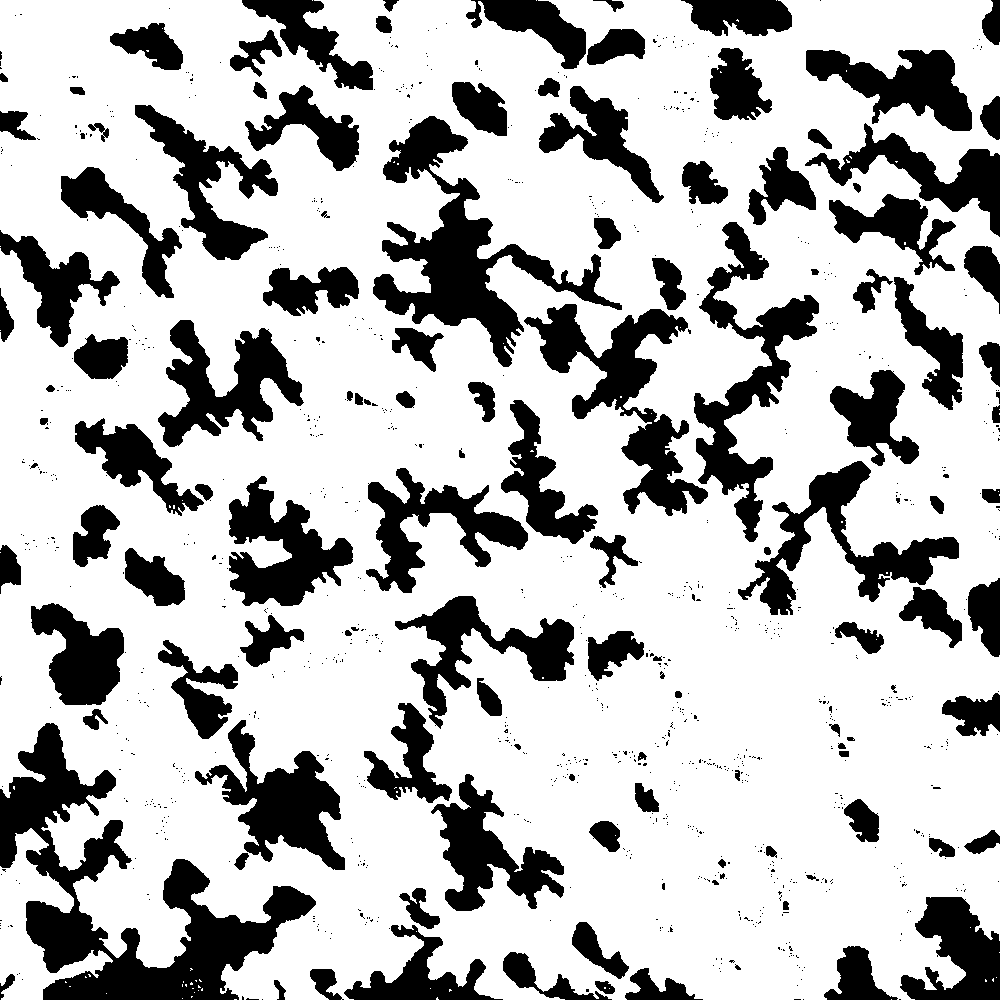
\includegraphics[width=0.3\textwidth]{../images/noise-all.png}
    \label{fig:noise-all}}
  \vskip\baselineskip
  \subfigure[Sandstone]{
    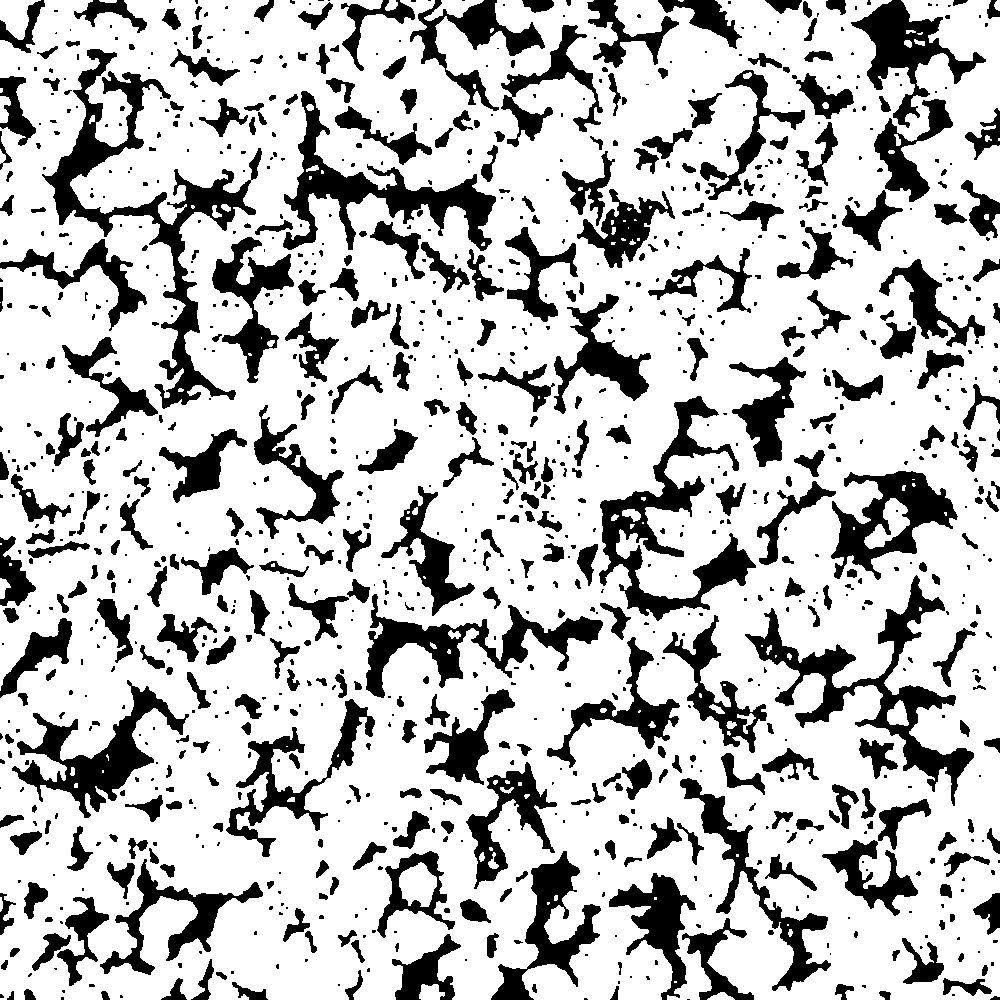
\includegraphics[width=0.3\textwidth]{../images/sandstone-orig.png}
    \label{fig:sandstone-orig}}
  \hfill
  \subfigure[Reconstruction of \cref{fig:sandstone-orig} using set 1]{
    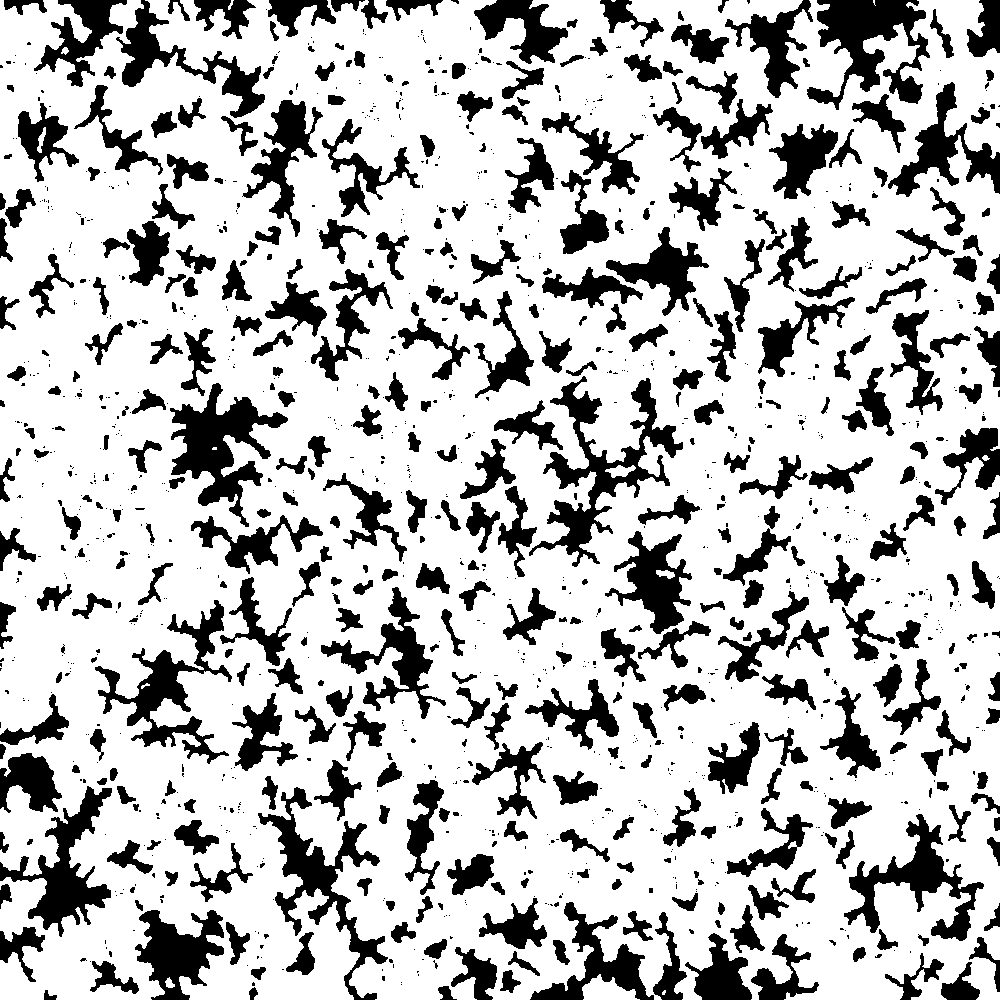
\includegraphics[width=0.3\textwidth]{../images/sandstone-s2l2.png}
    \label{fig:sandstone-s2l2}}
  \hfill
  \subfigure[Reconstruction of \cref{fig:sandstone-orig} using set 2]{
    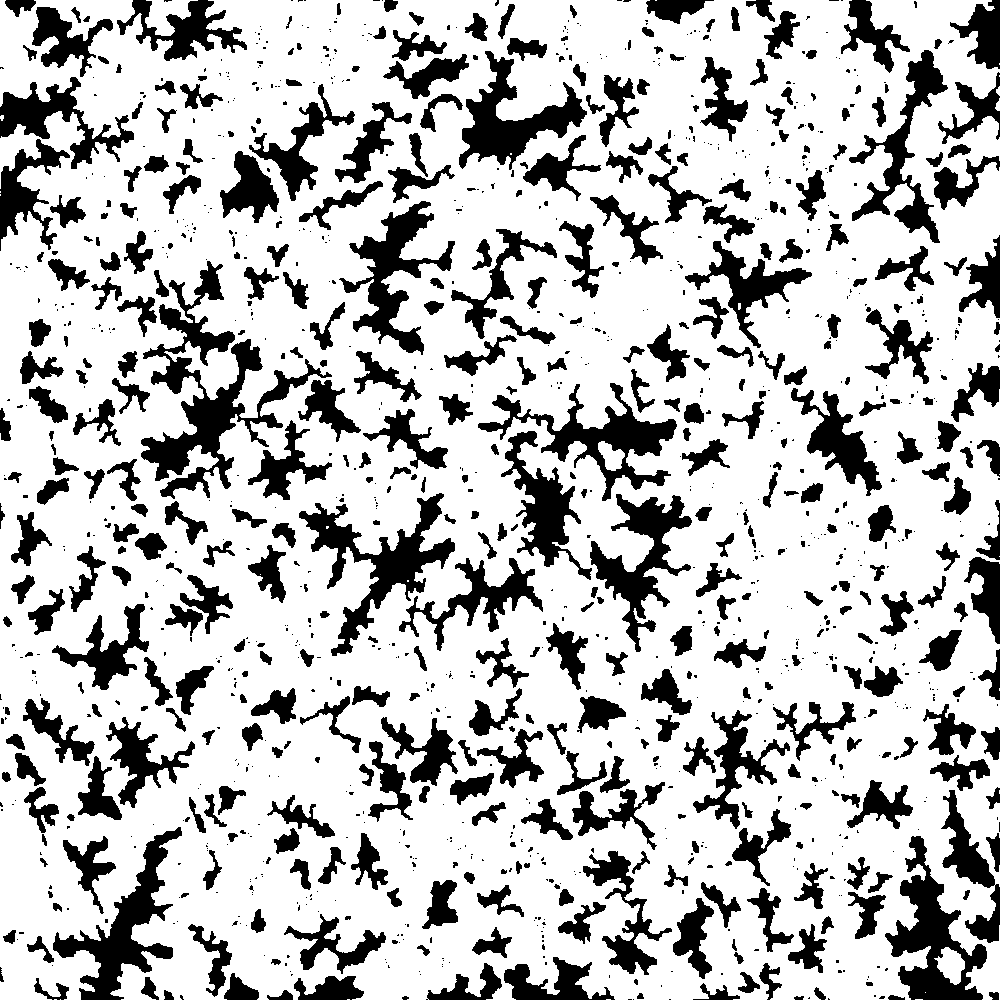
\includegraphics[width=0.3\textwidth]{../images/sandstone-all.png}
    \label{fig:sandstone-all}}
  \caption[]{Original images and their reconstructions (continued)}
  \label{fig:orig-recon2}
\end{figure*}

\begin{figure*}[htp]
  \centering
  \subfigure[]{
    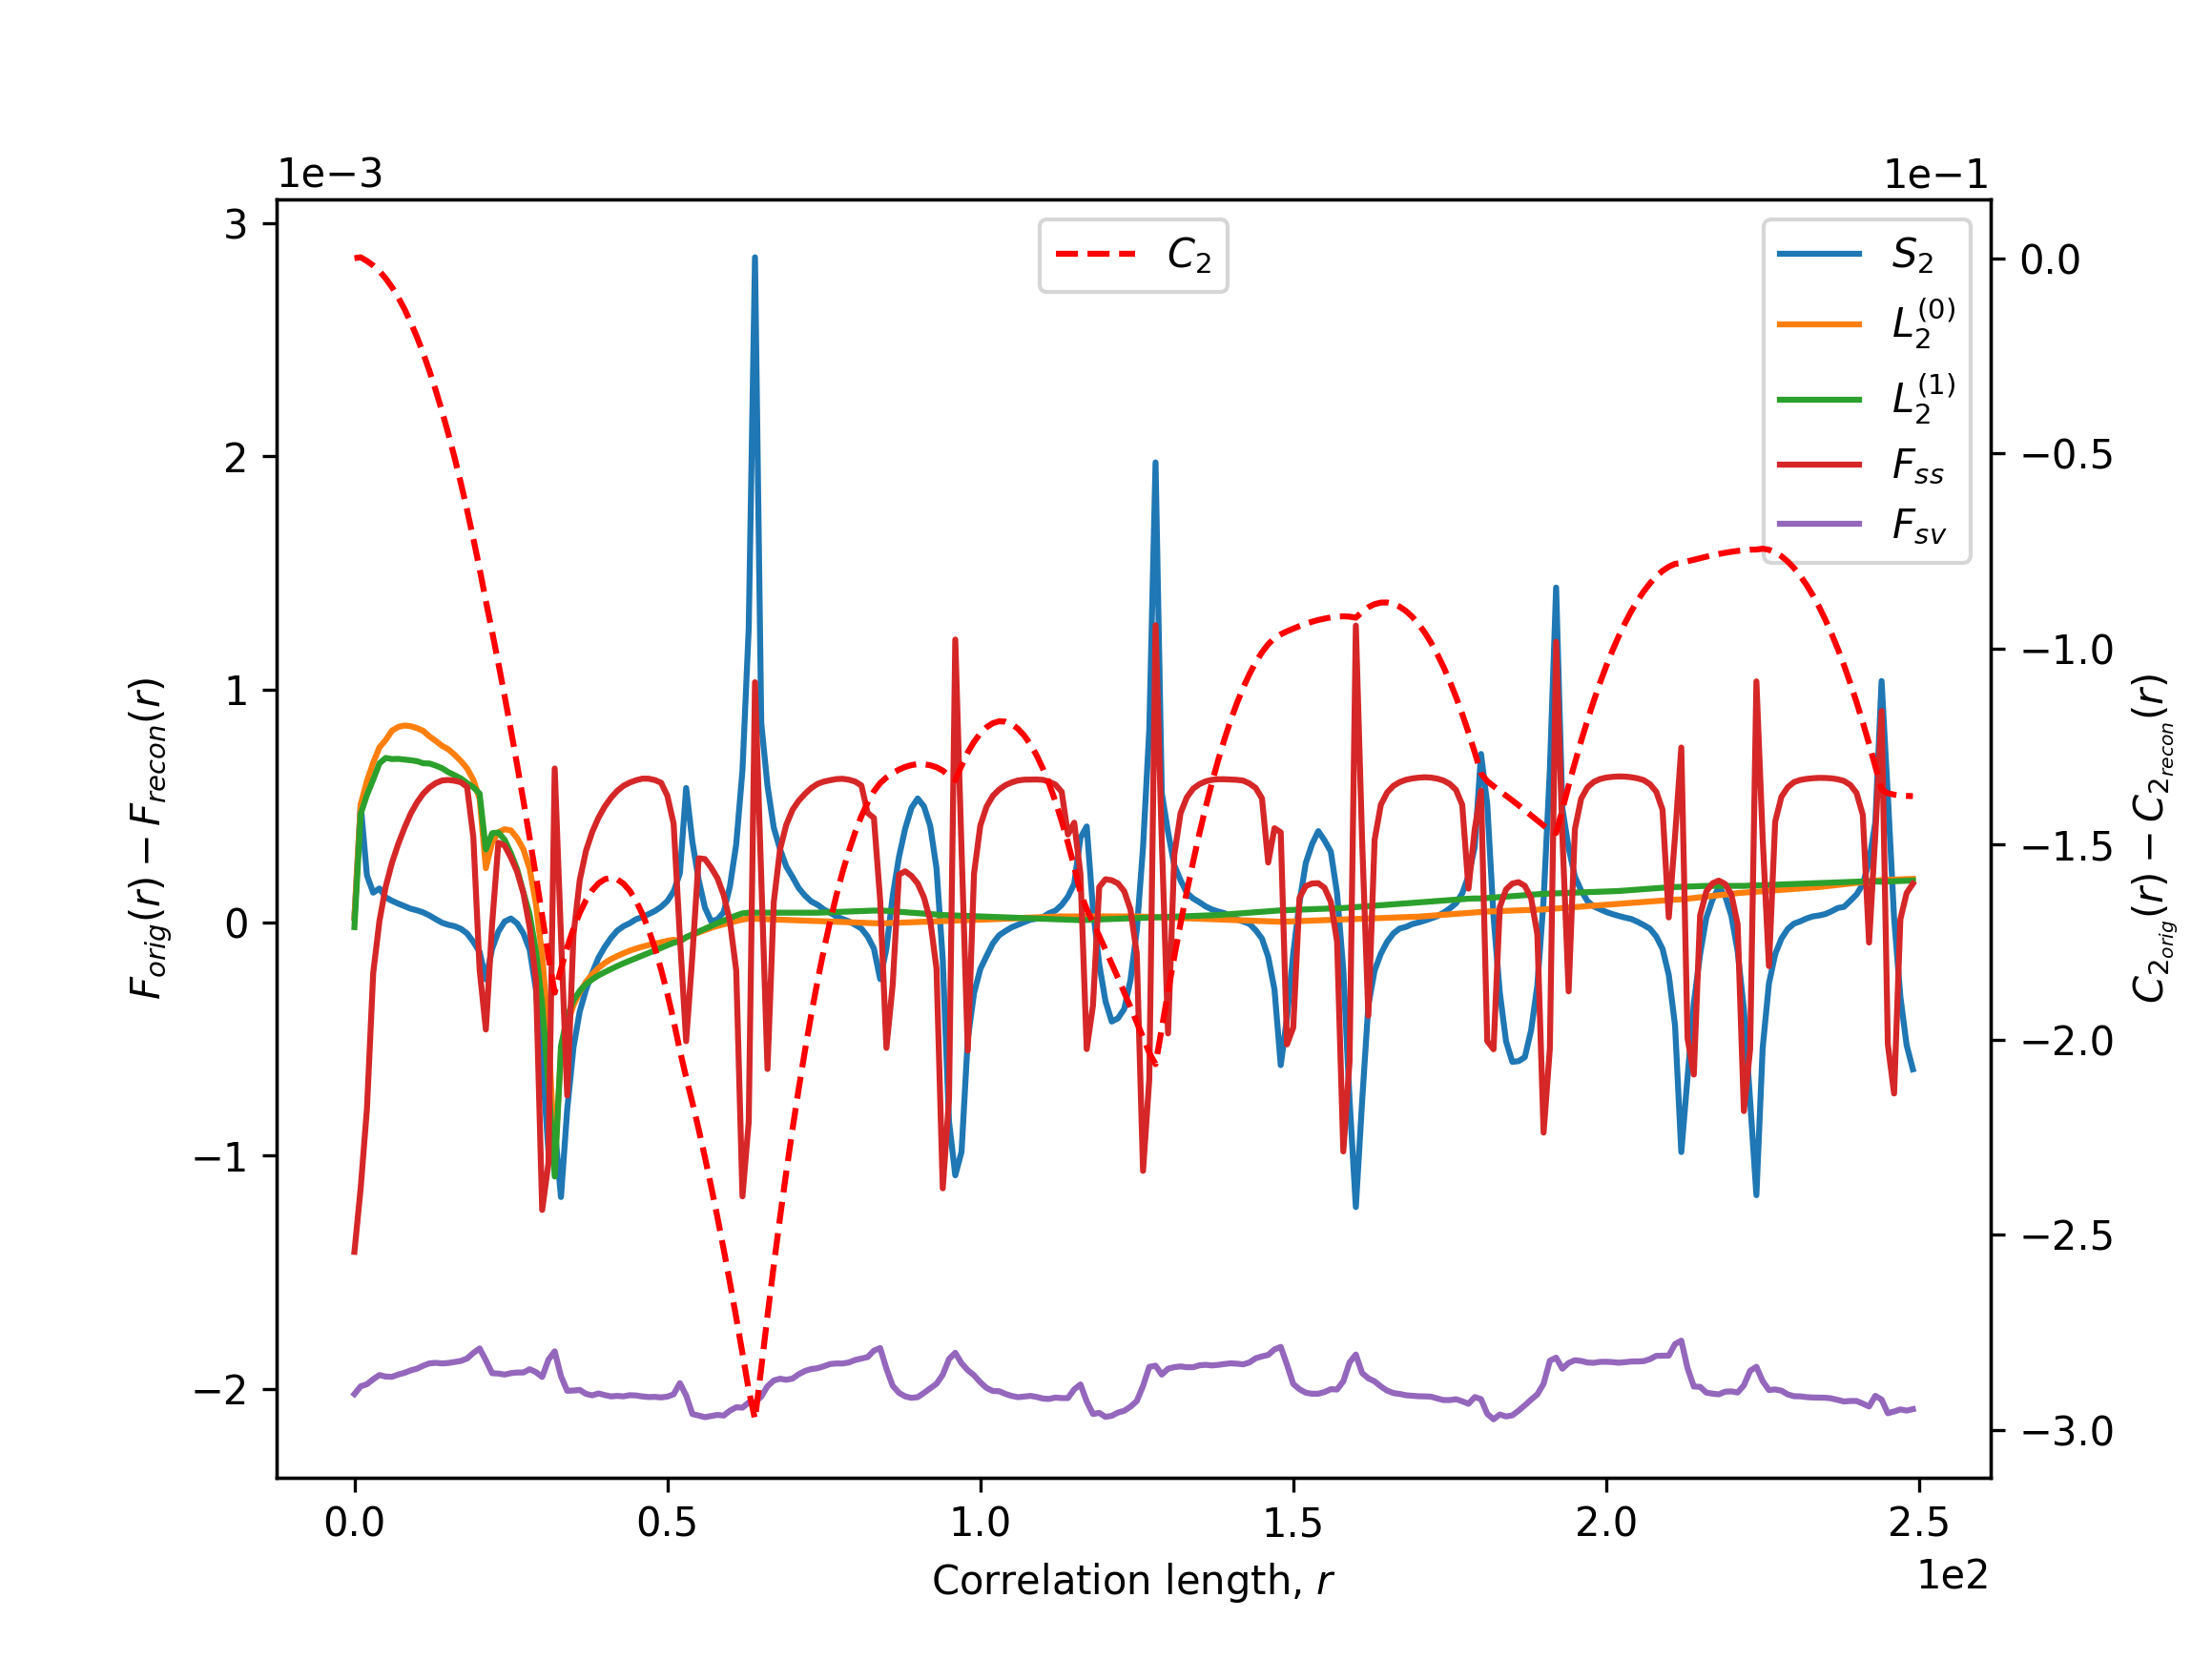
\includegraphics[width=0.3\textwidth]{../corrfns-plots/checkboard-s2l2.png}
    \label{fig:check-corr-s2l2}}
  \hfill
  \subfigure[]{
    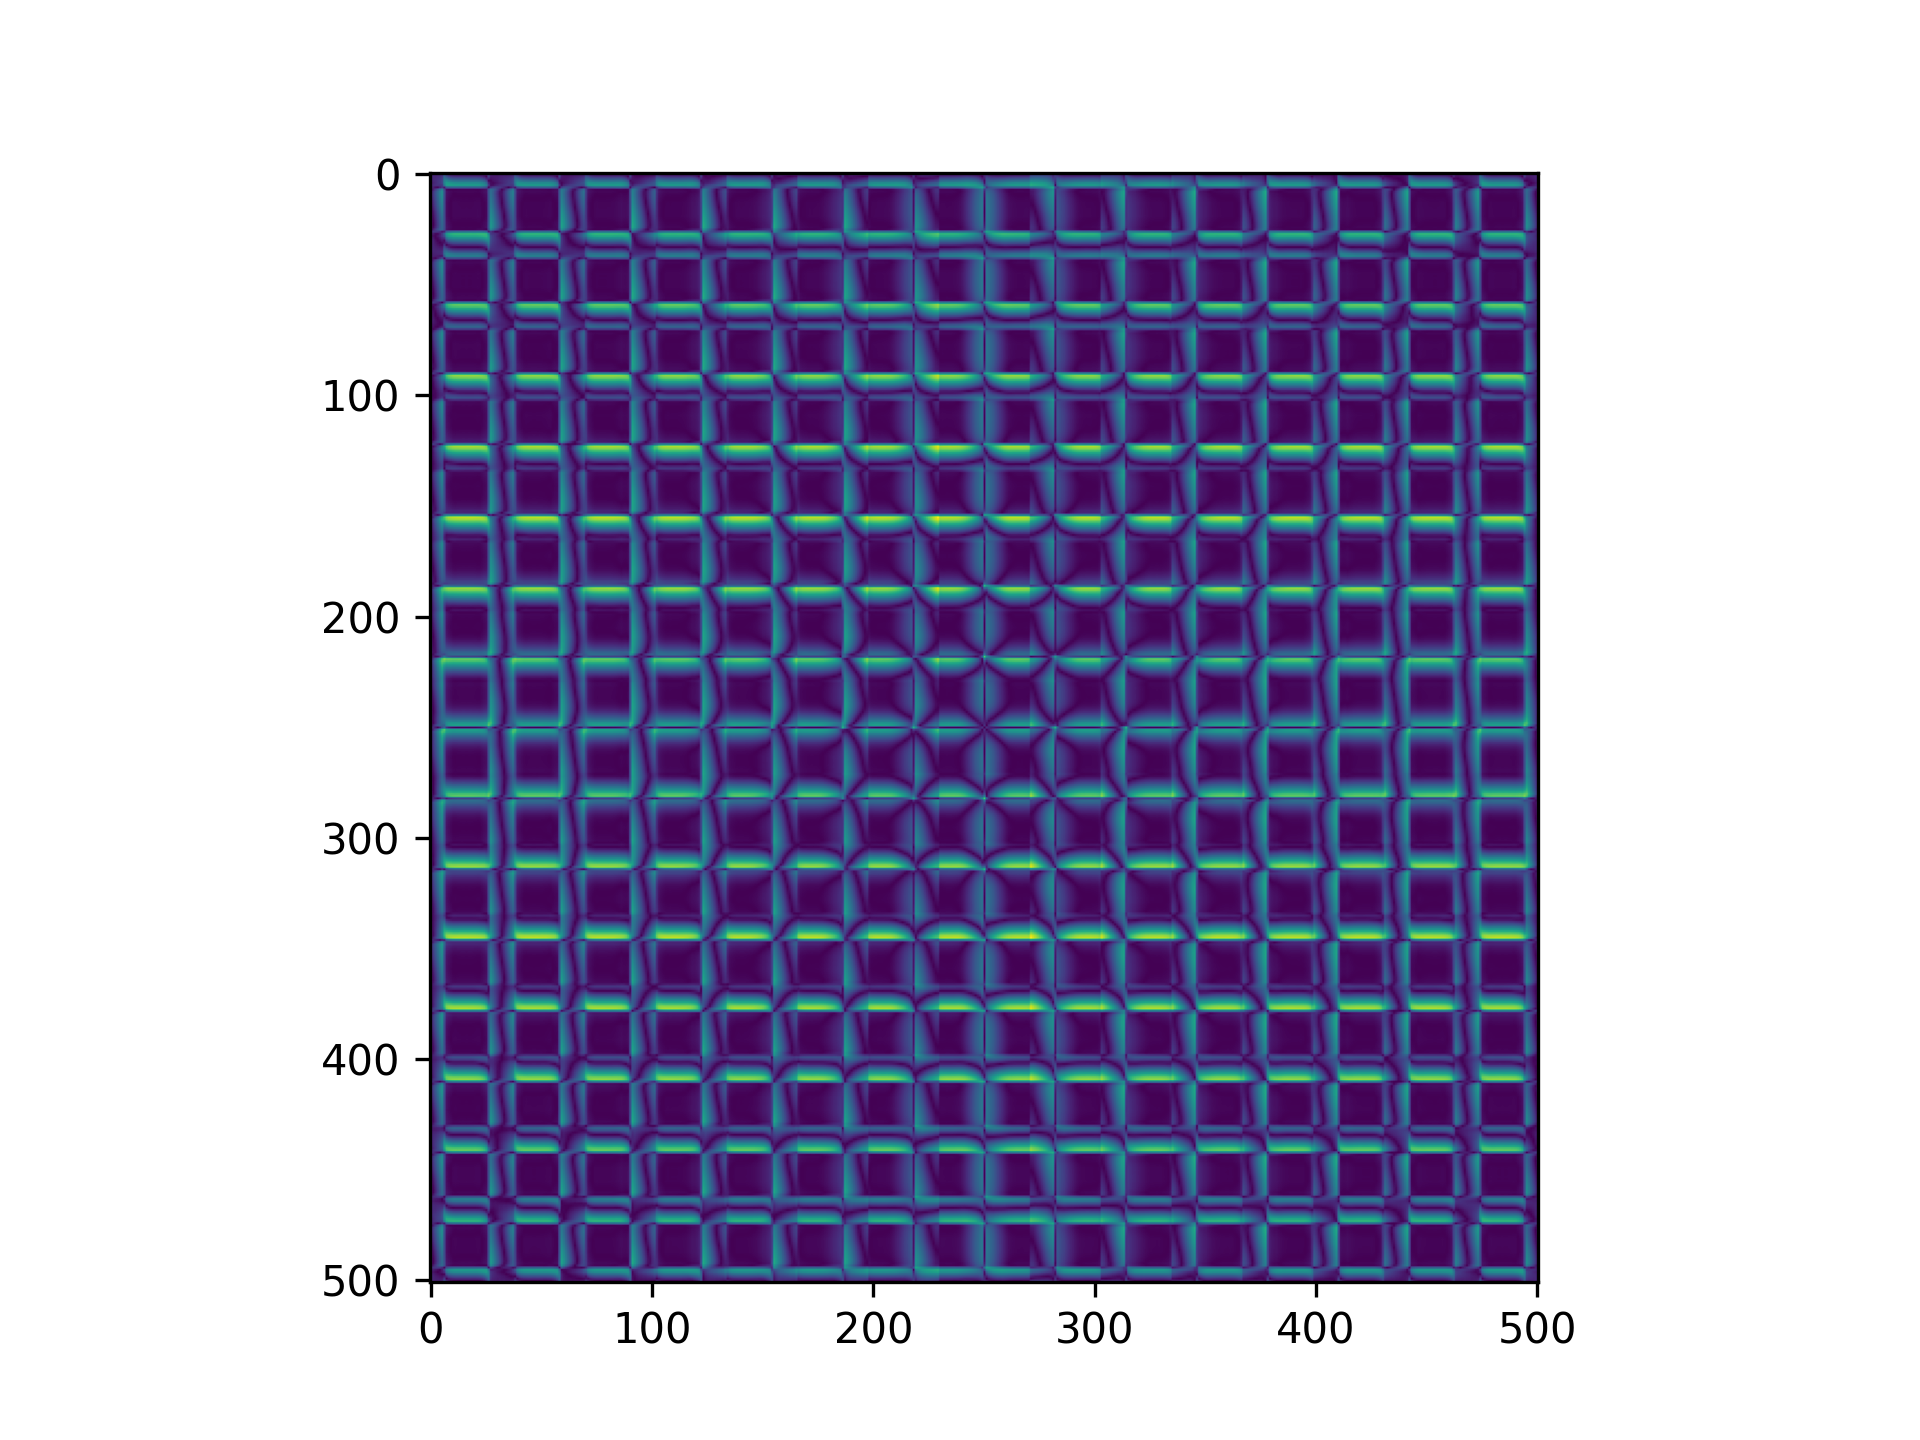
\includegraphics[width=0.3\textwidth]{../corrfns-plots/checkboard-s2l2-map.png}
    \label{fig:check-corr-map}}
  \hfill
  \subfigure[]{
    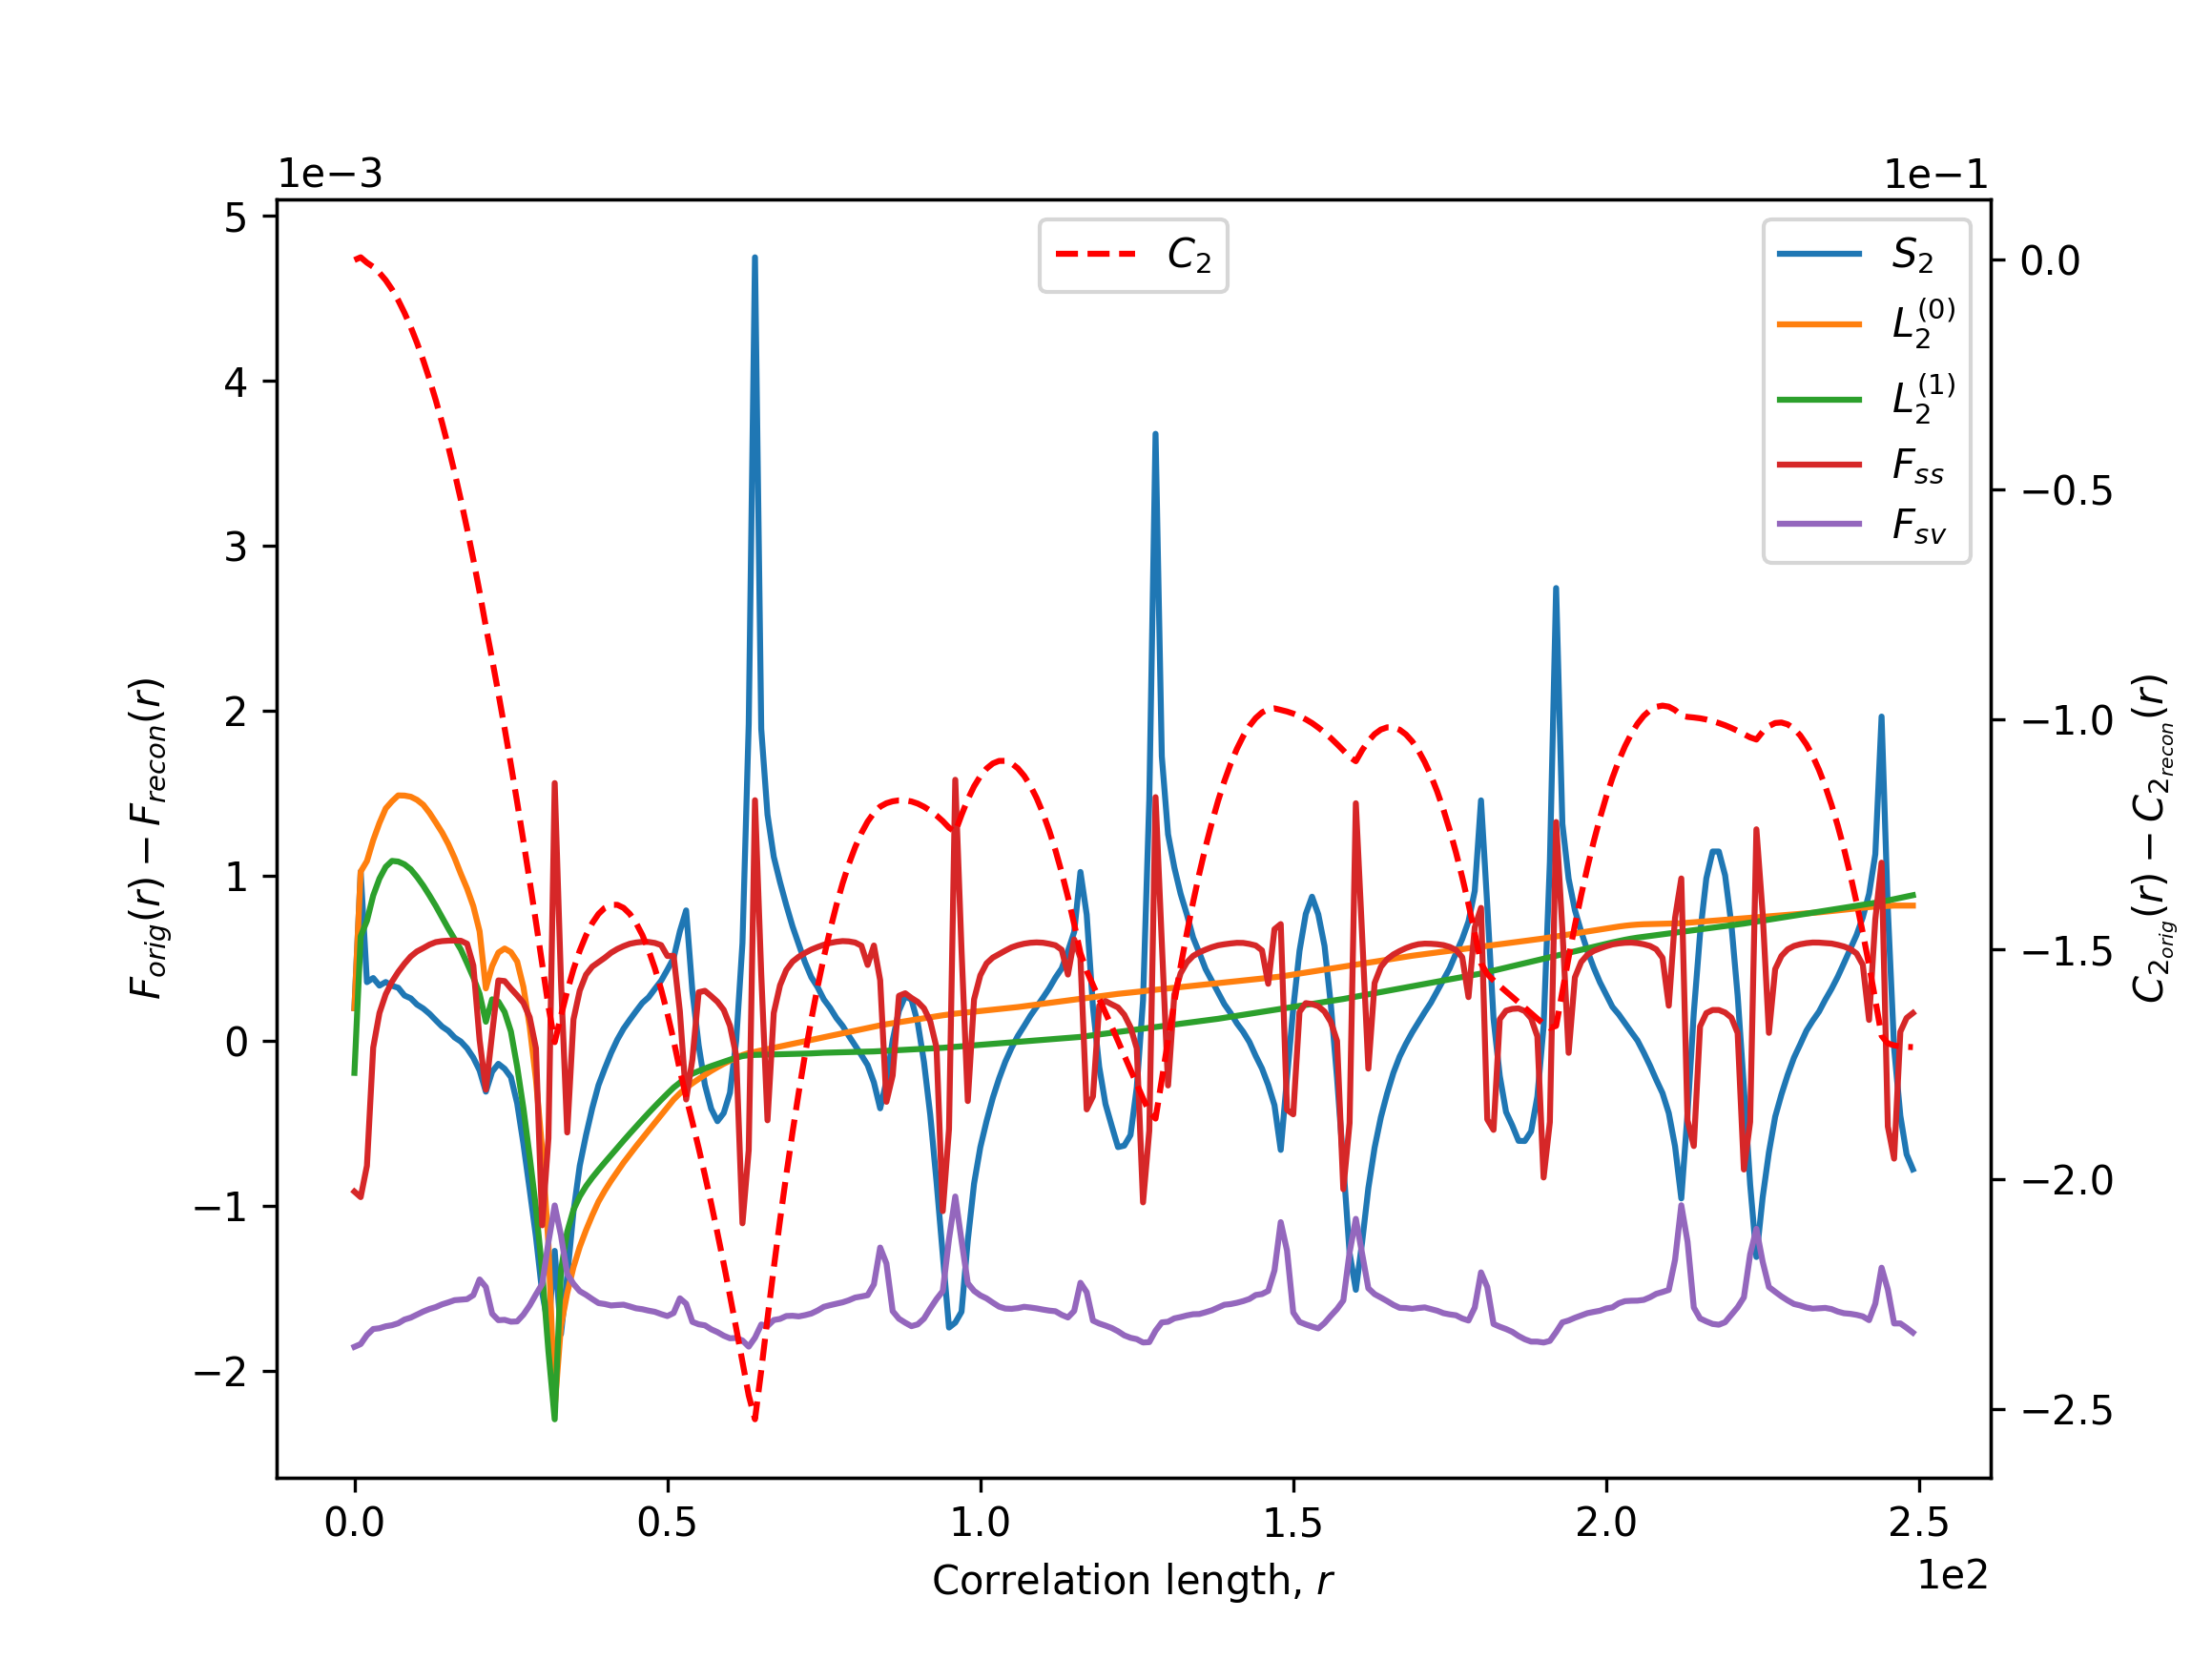
\includegraphics[width=0.3\textwidth]{../corrfns-plots/checkboard-all.png}
    \label{fig:check-corr-all}}
  \vskip\baselineskip
  \subfigure[]{
    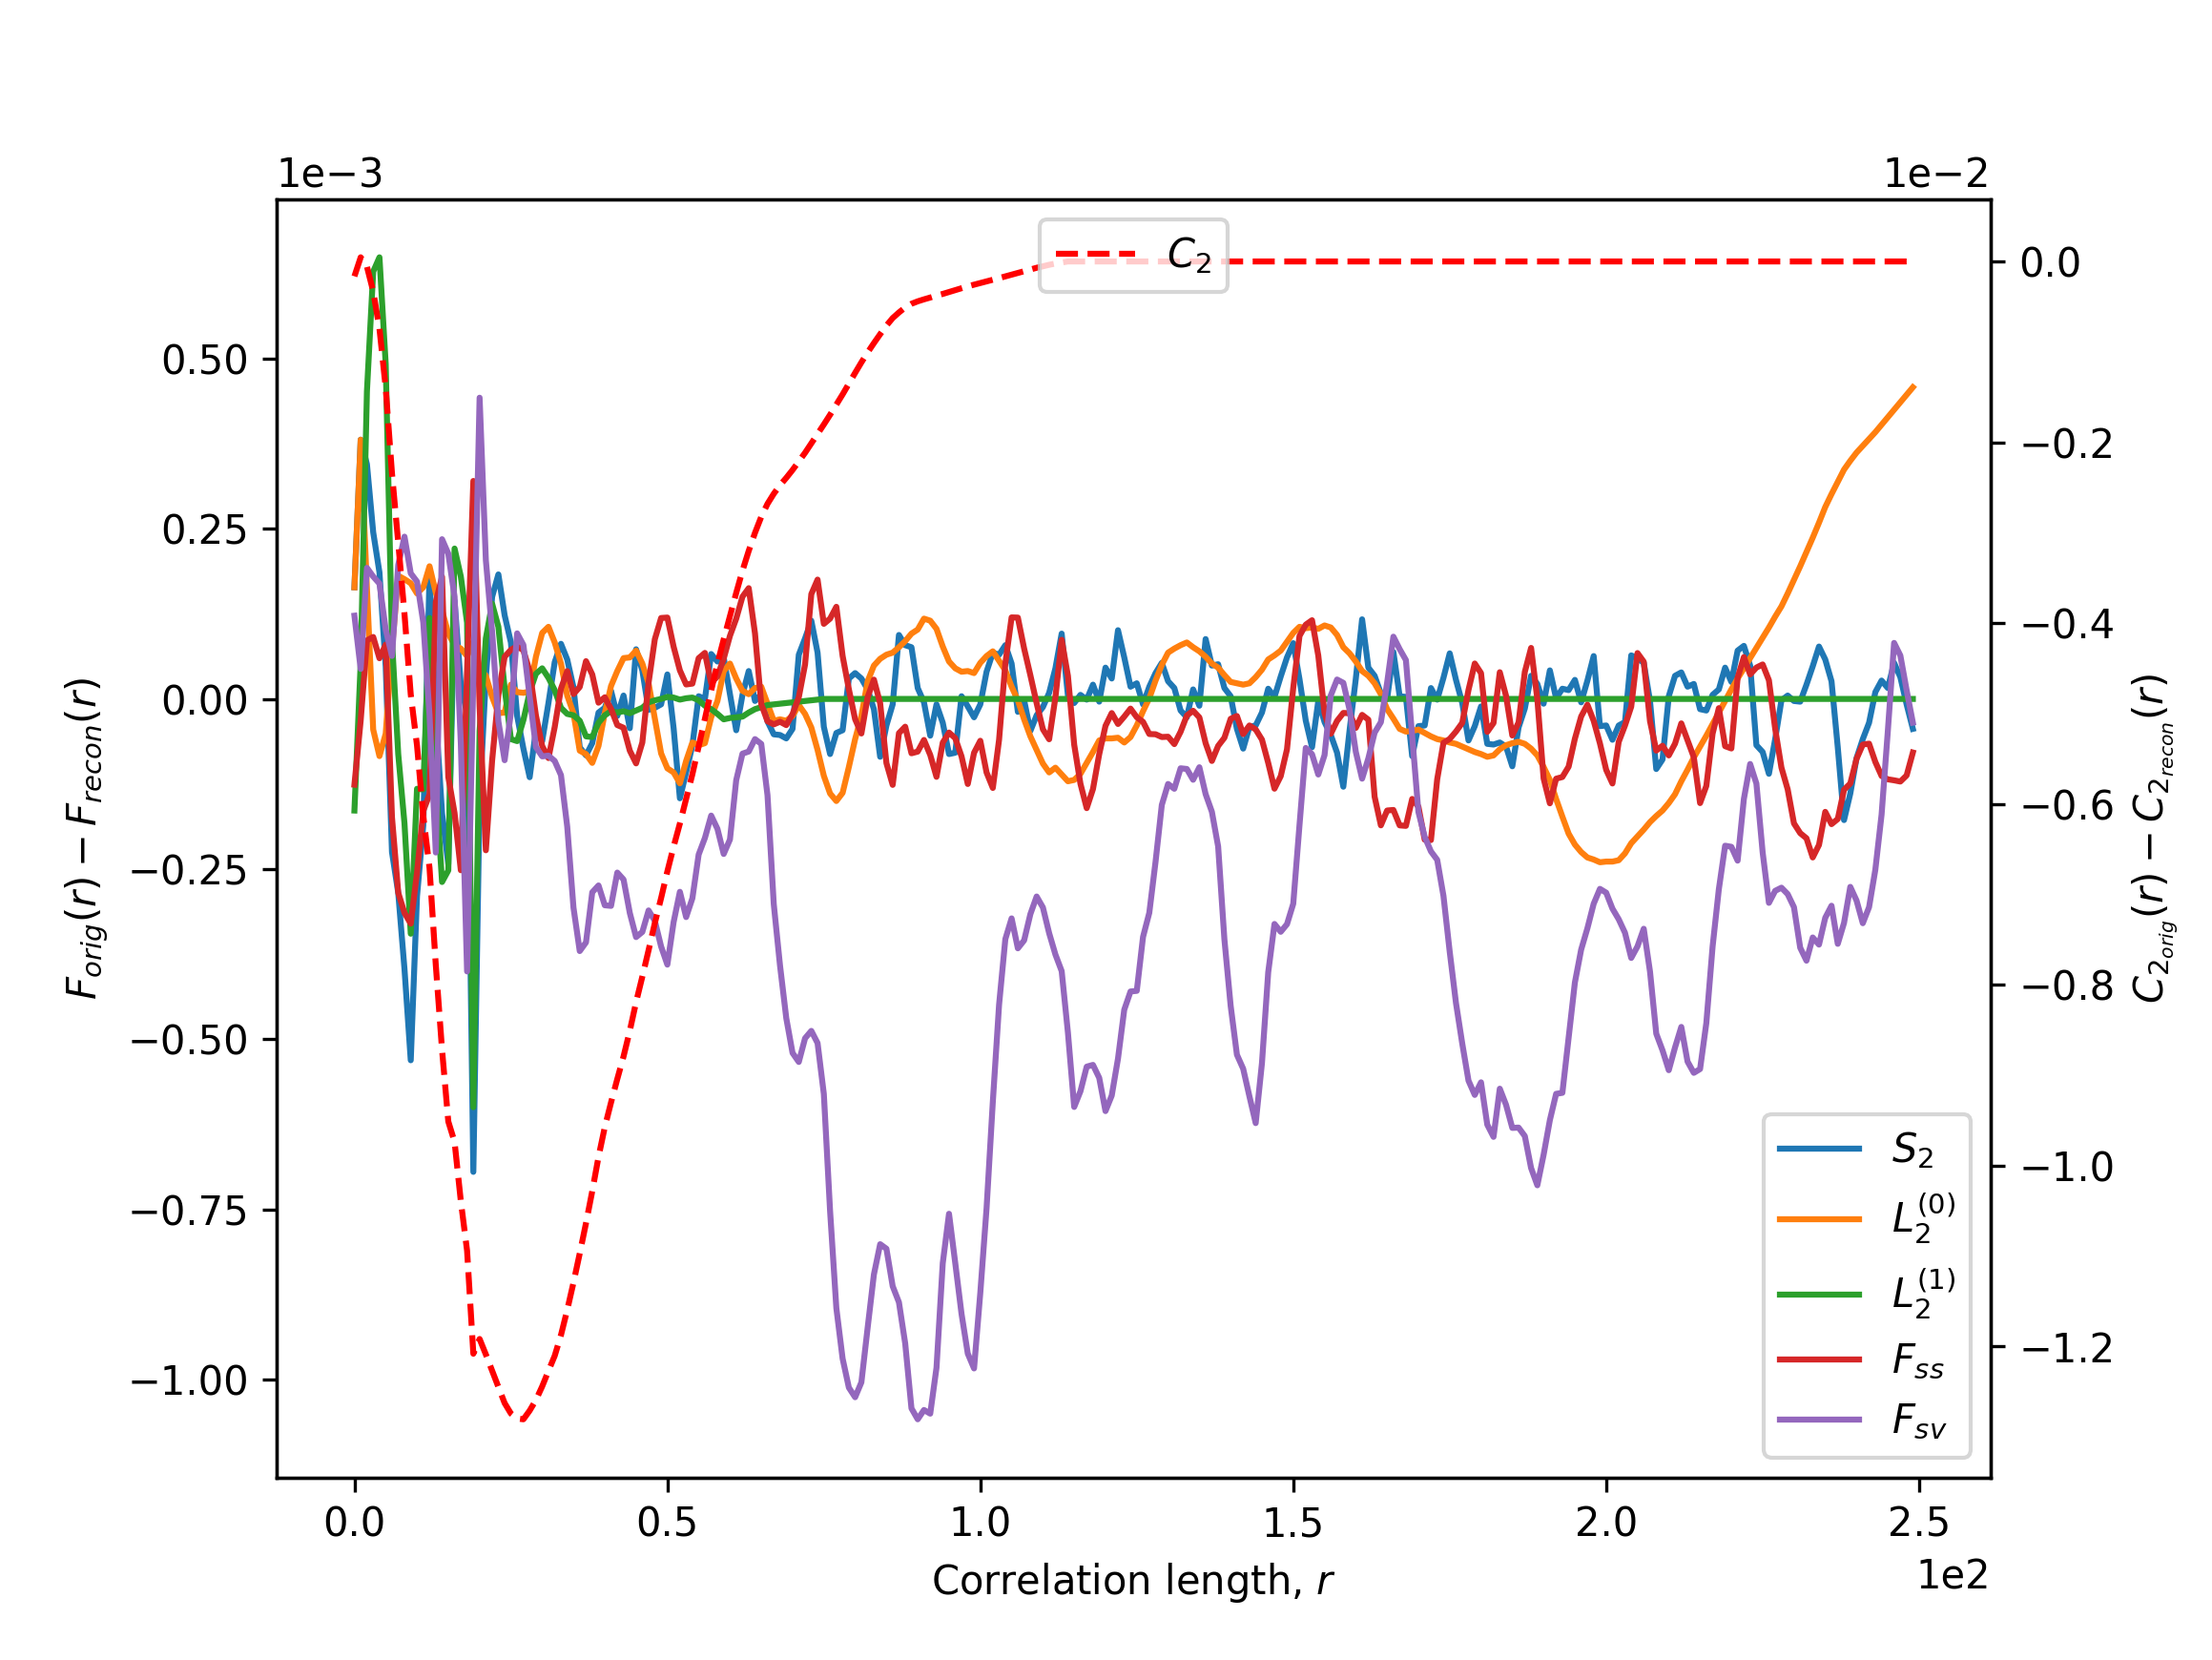
\includegraphics[width=0.3\textwidth]{../corrfns-plots/disks-s2l2.png}
    \label{fig:disks-corr-s2l2}}
  \hfill
  \subfigure[]{
    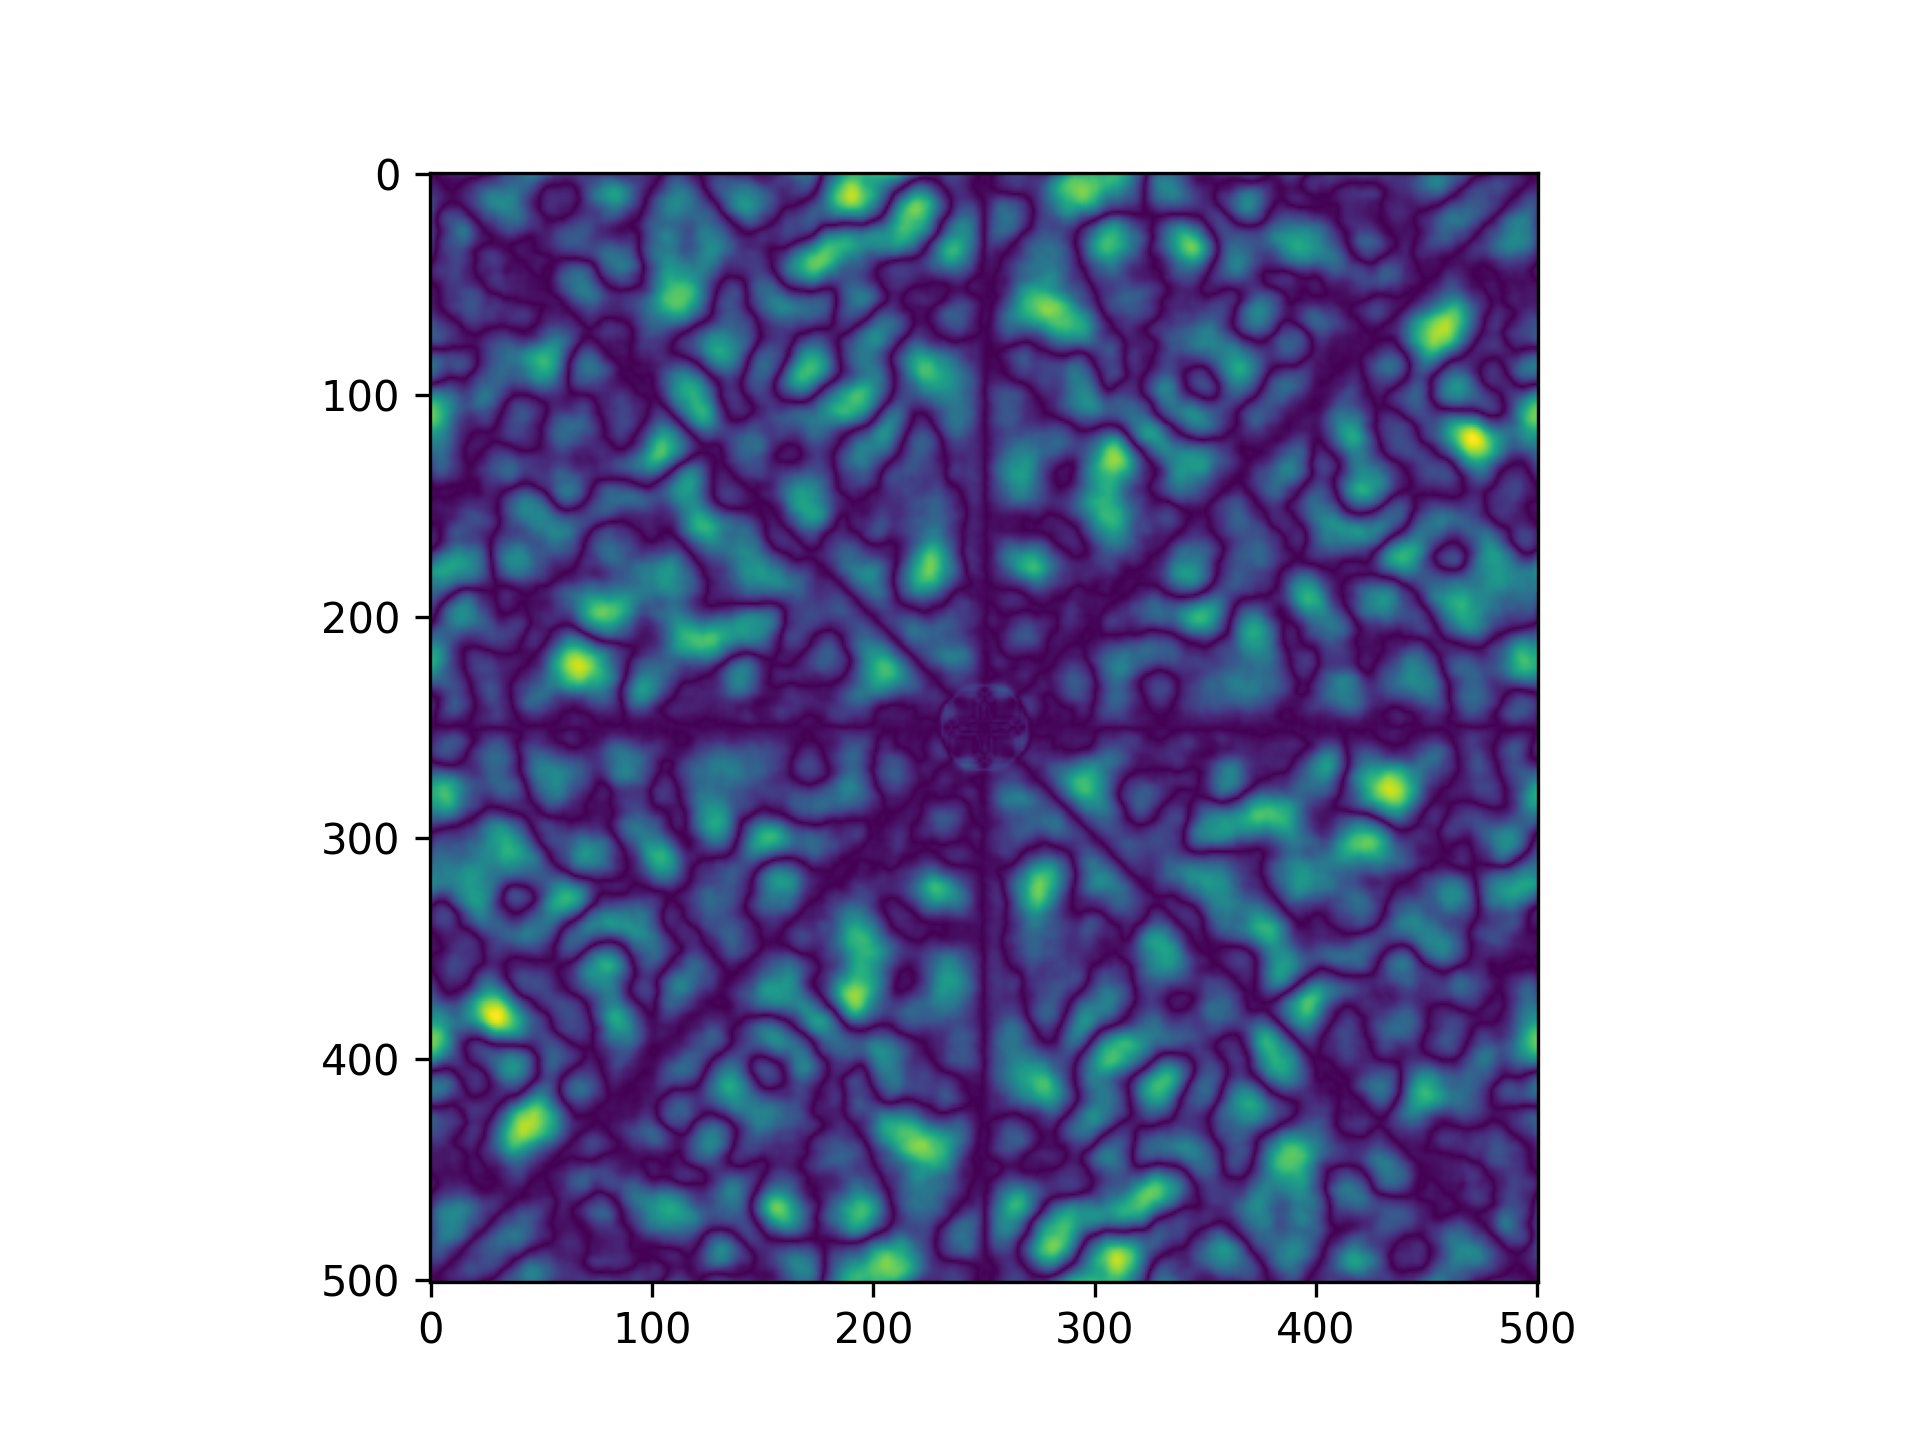
\includegraphics[width=0.3\textwidth]{../corrfns-plots/disks-s2l2-map.png}
    \label{fig:disks-corr-map}}
  \hfill
  \subfigure[]{
    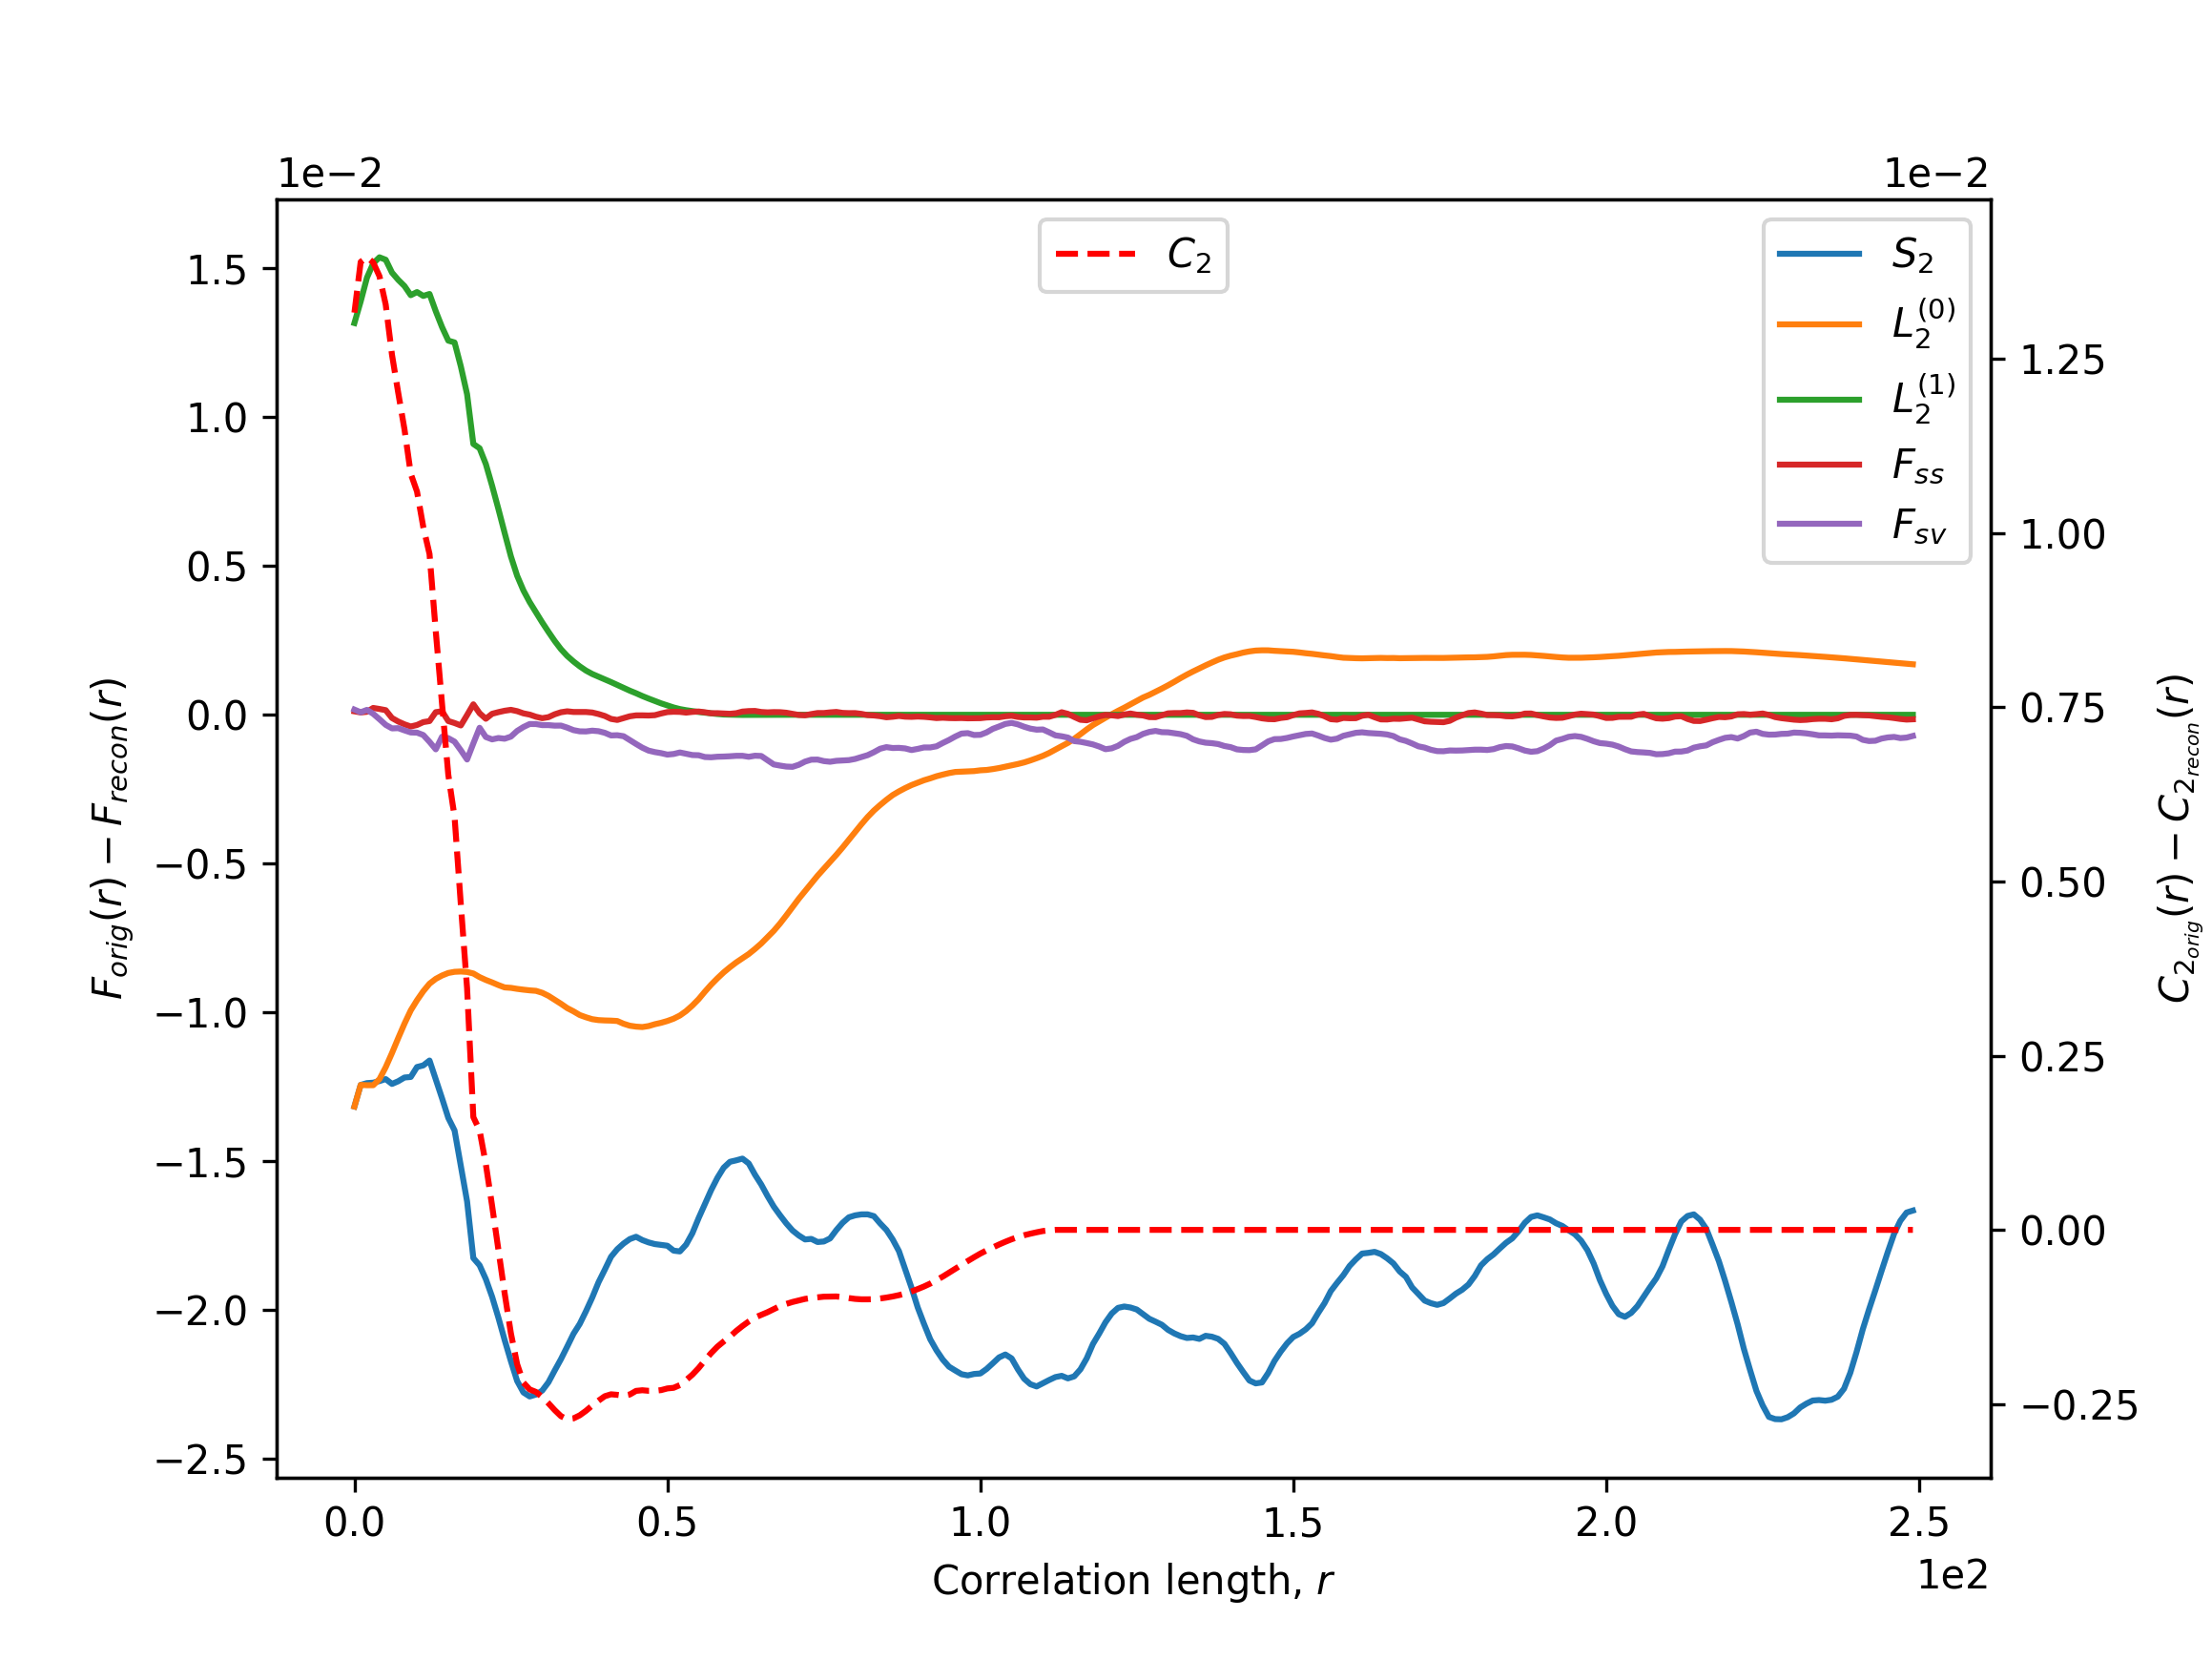
\includegraphics[width=0.3\textwidth]{../corrfns-plots/disks-all.png}
    \label{fig:disks-corr-all}}
  \caption[]{Difference between correlation functions of the original and
    reconstructed images. From \cref{fig:check-corr-s2l2} to
    \cref{fig:check-corr-all} — checkerboard, from \cref{fig:disks-corr-s2l2} to
    \cref{fig:disks-corr-all} — overlapping disks. Images to the left are
    for reconstructions using correlation functions from the first set, images
    to the right are for reconstructions using functions from the second
    set. Images in the center are differences between two-point correlation maps
    of the original and reconstructed images.}
  \label{fig:corrfn-diff1}
\end{figure*}

\begin{figure*}[htp]
  \centering
  \subfigure[]{
    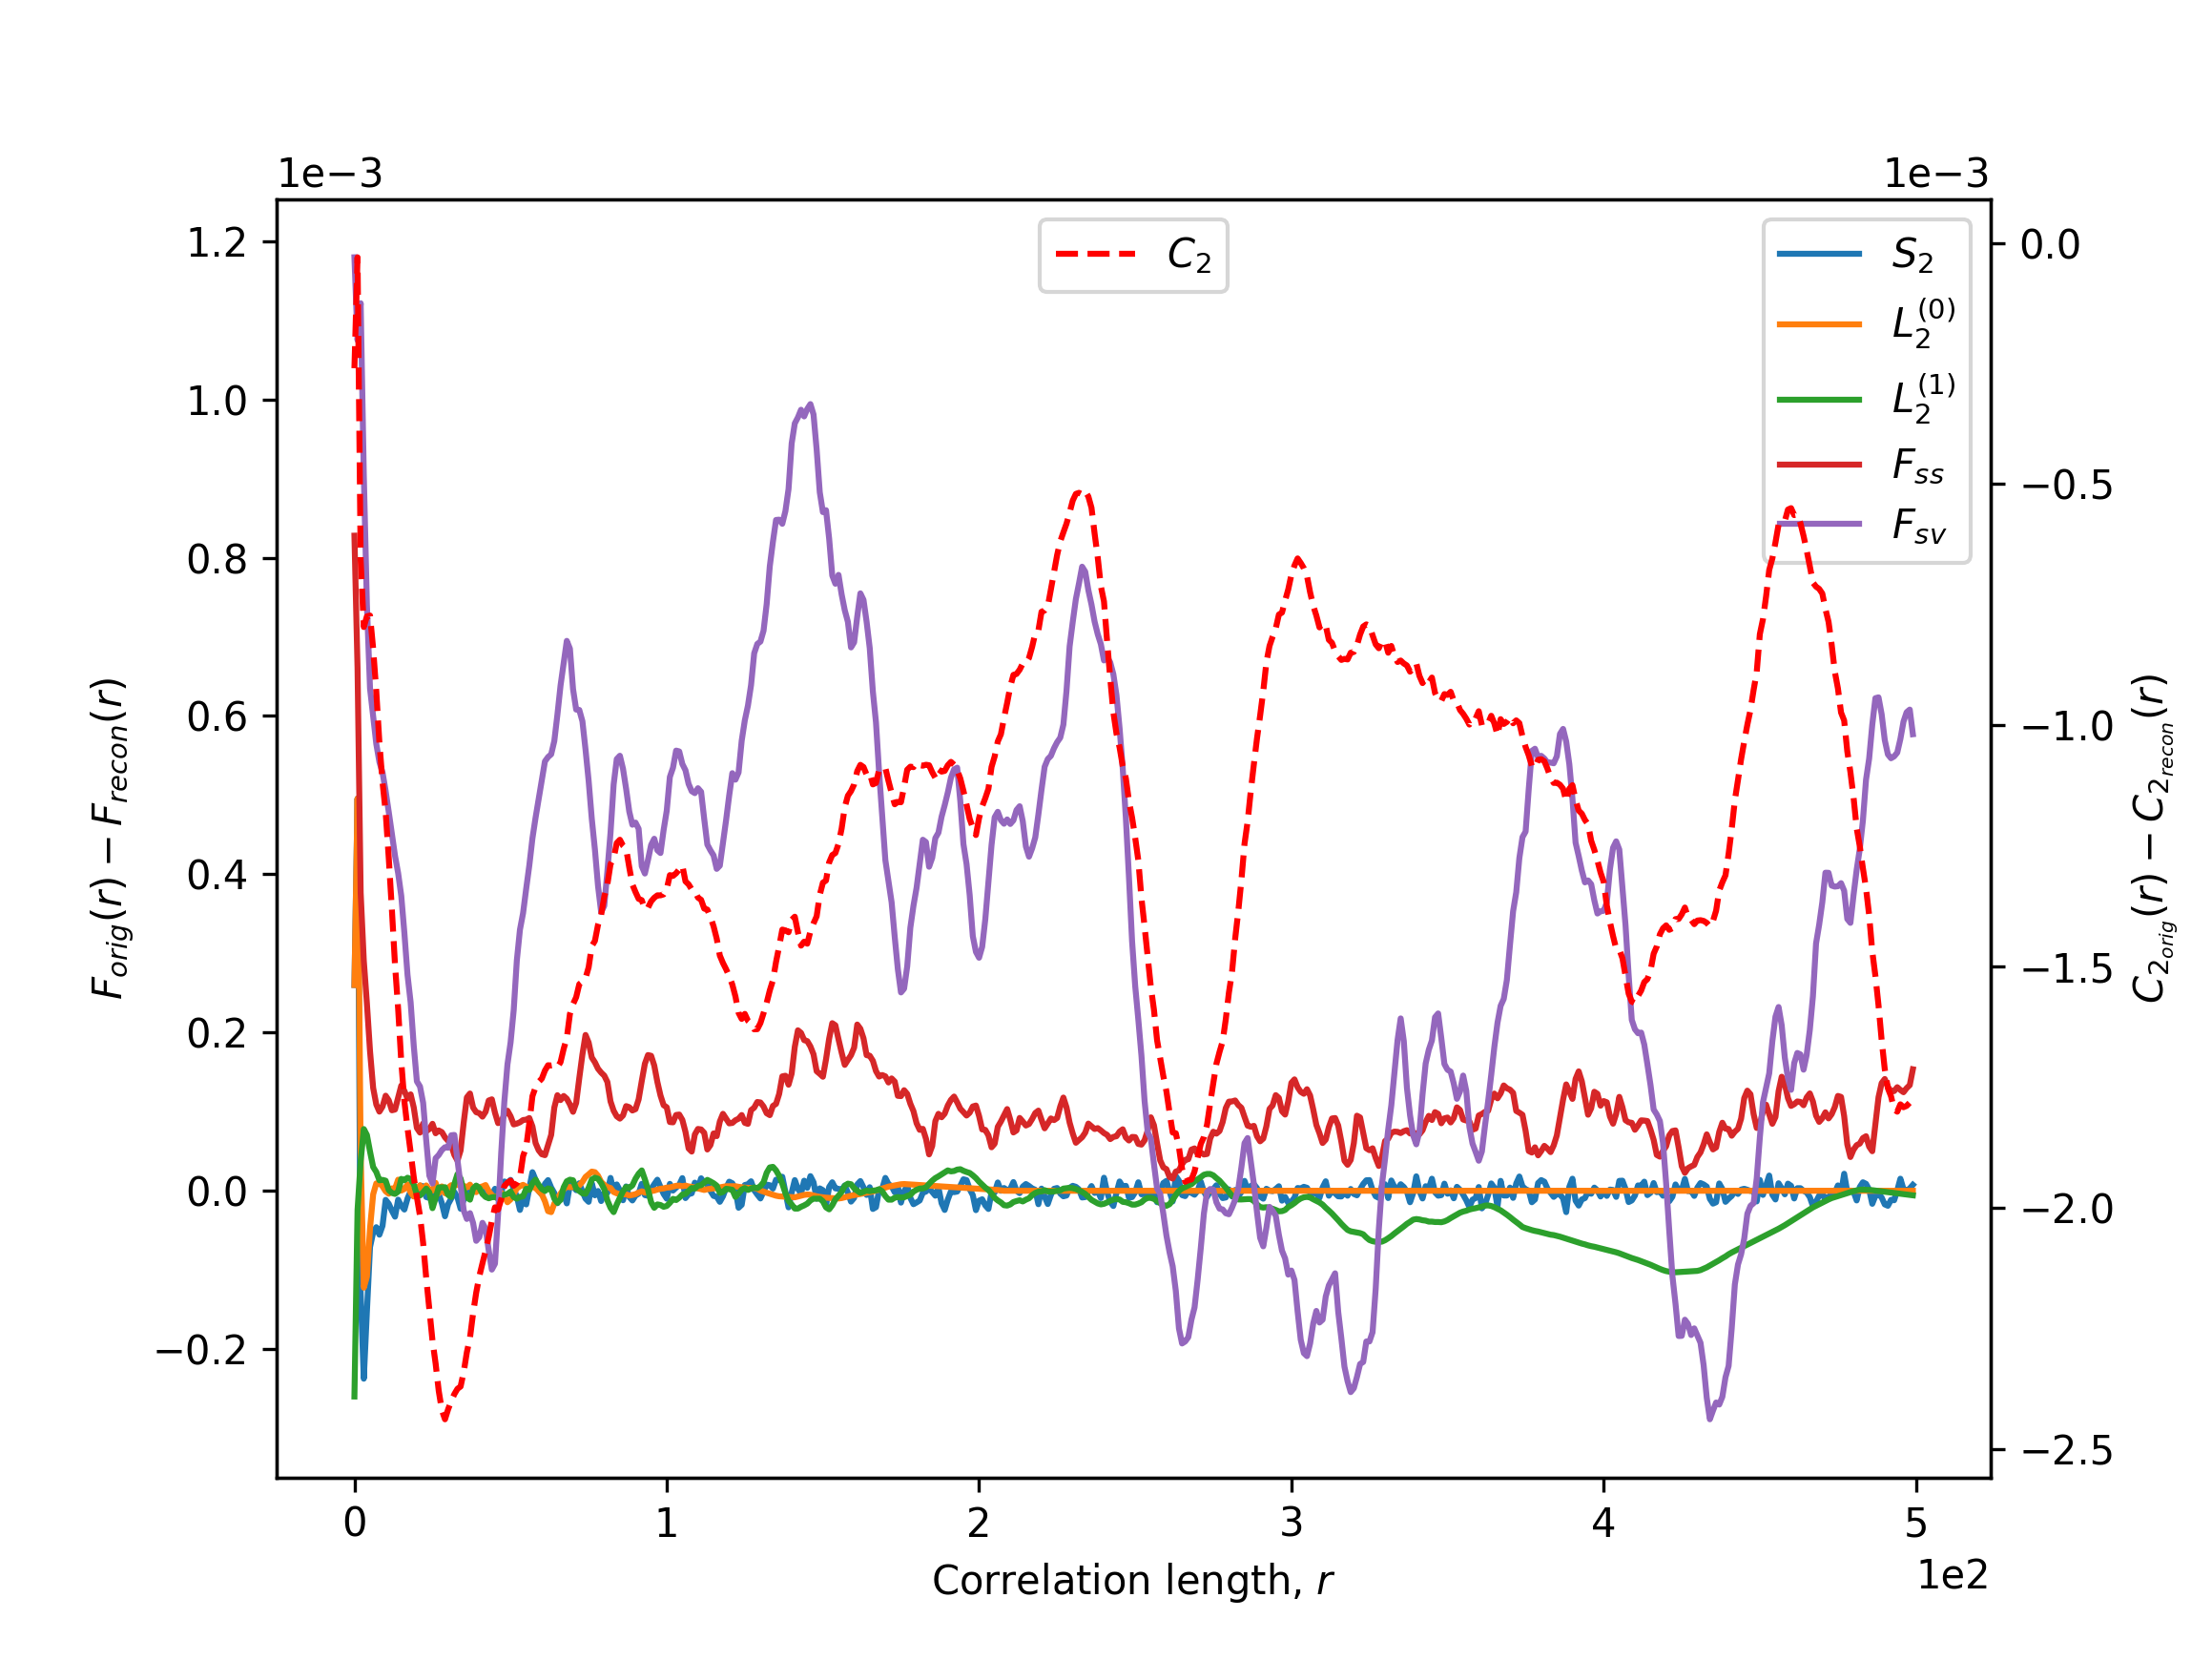
\includegraphics[width=0.3\textwidth]{../corrfns-plots/noise-s2l2.png}
    \label{fig:noise-corr-s2l2}}
  \hfill
  \subfigure[]{
    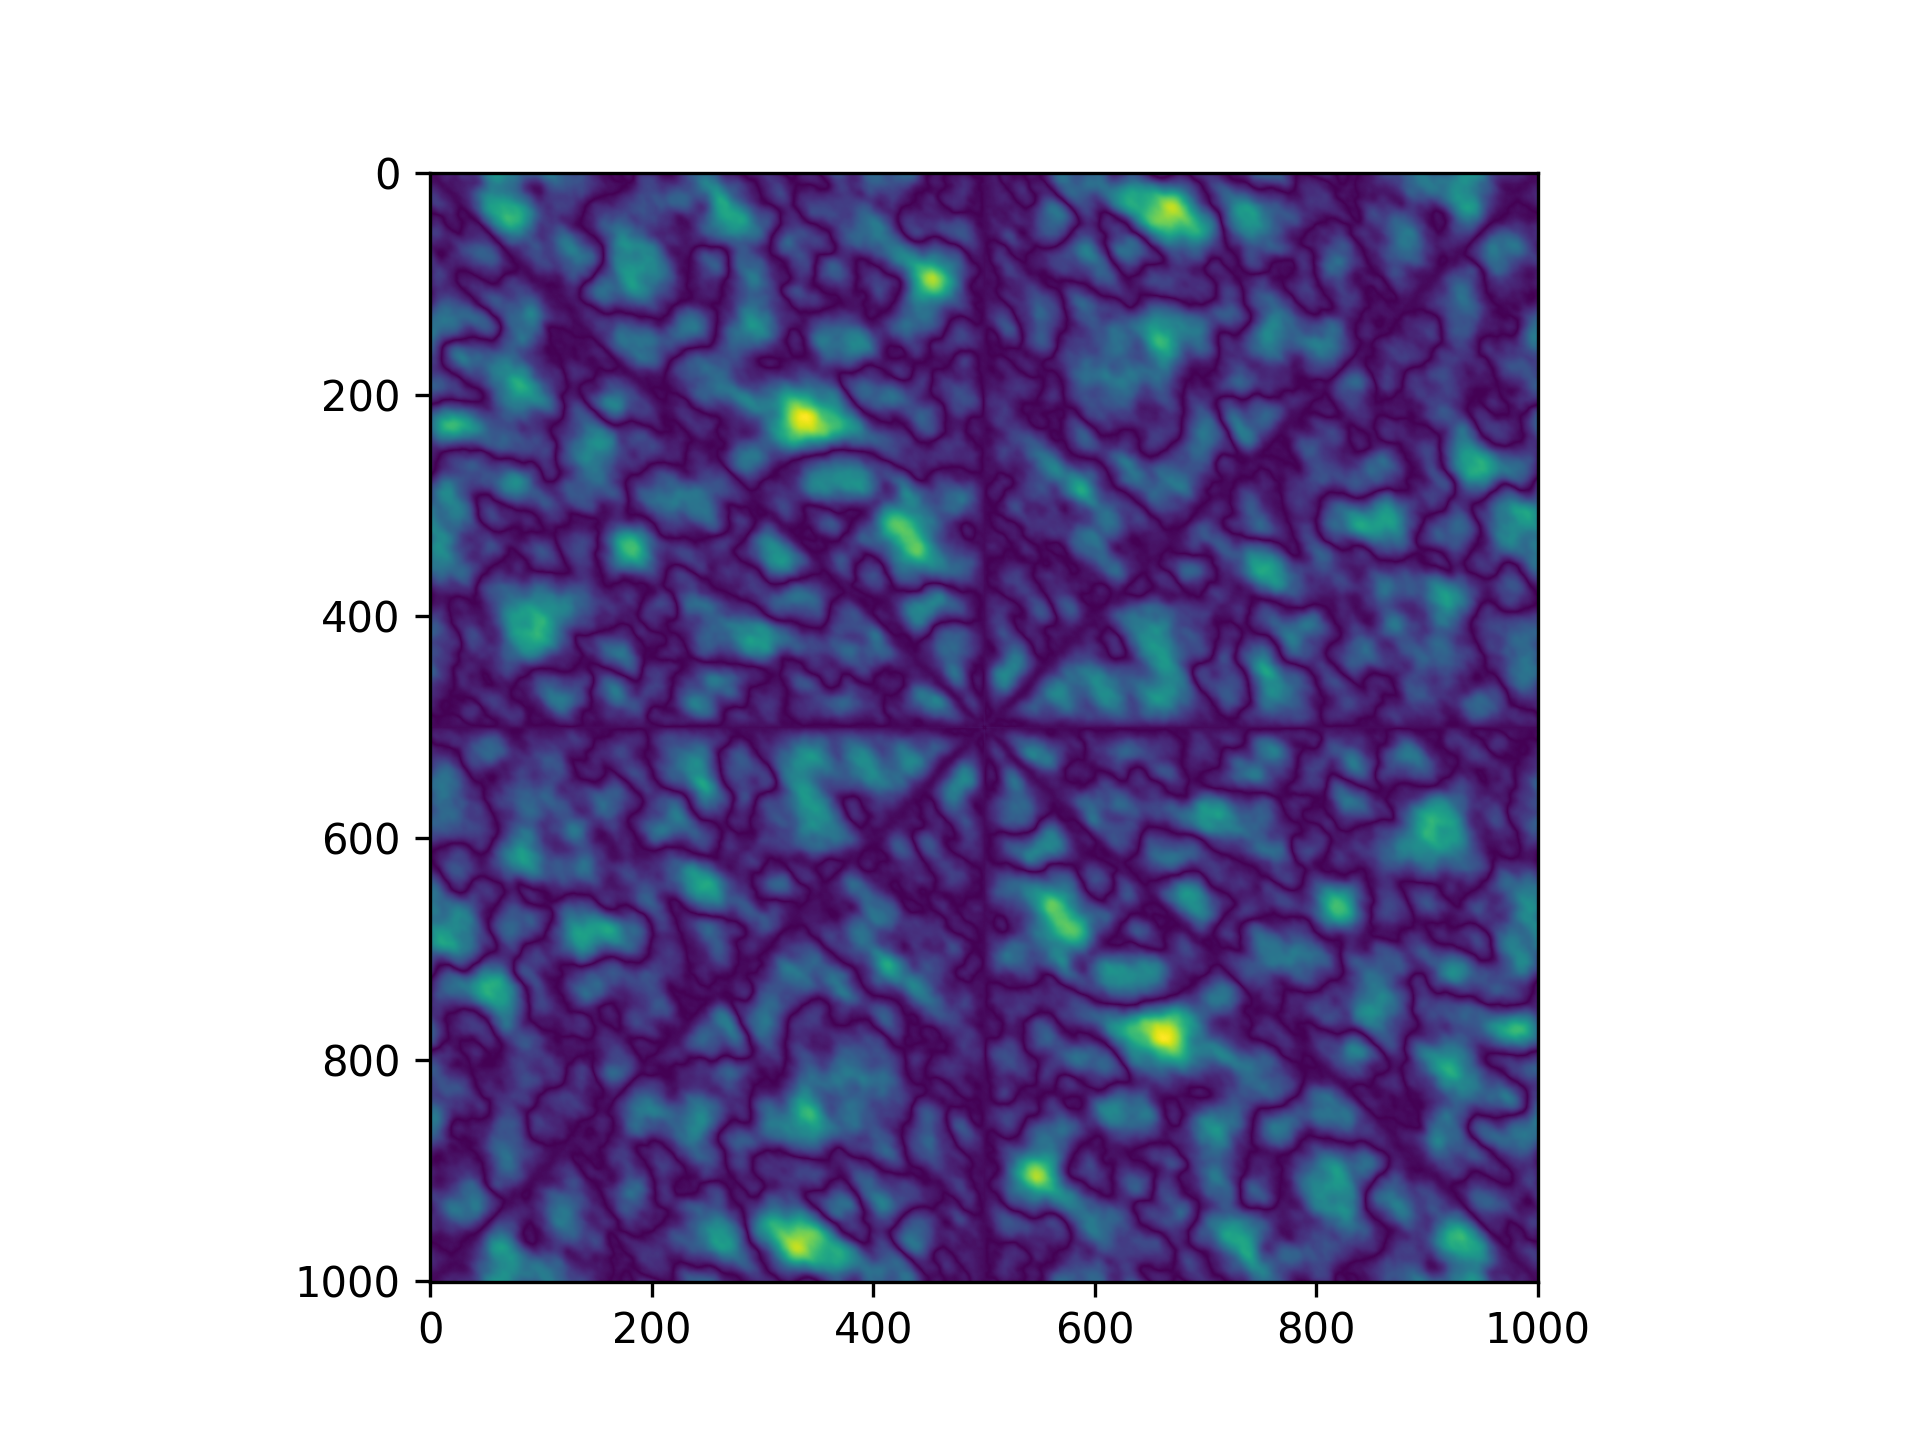
\includegraphics[width=0.3\textwidth]{../corrfns-plots/noise-s2l2-map.png}
    \label{fig:noise-corr-map}}
  \hfill
  \subfigure[]{
    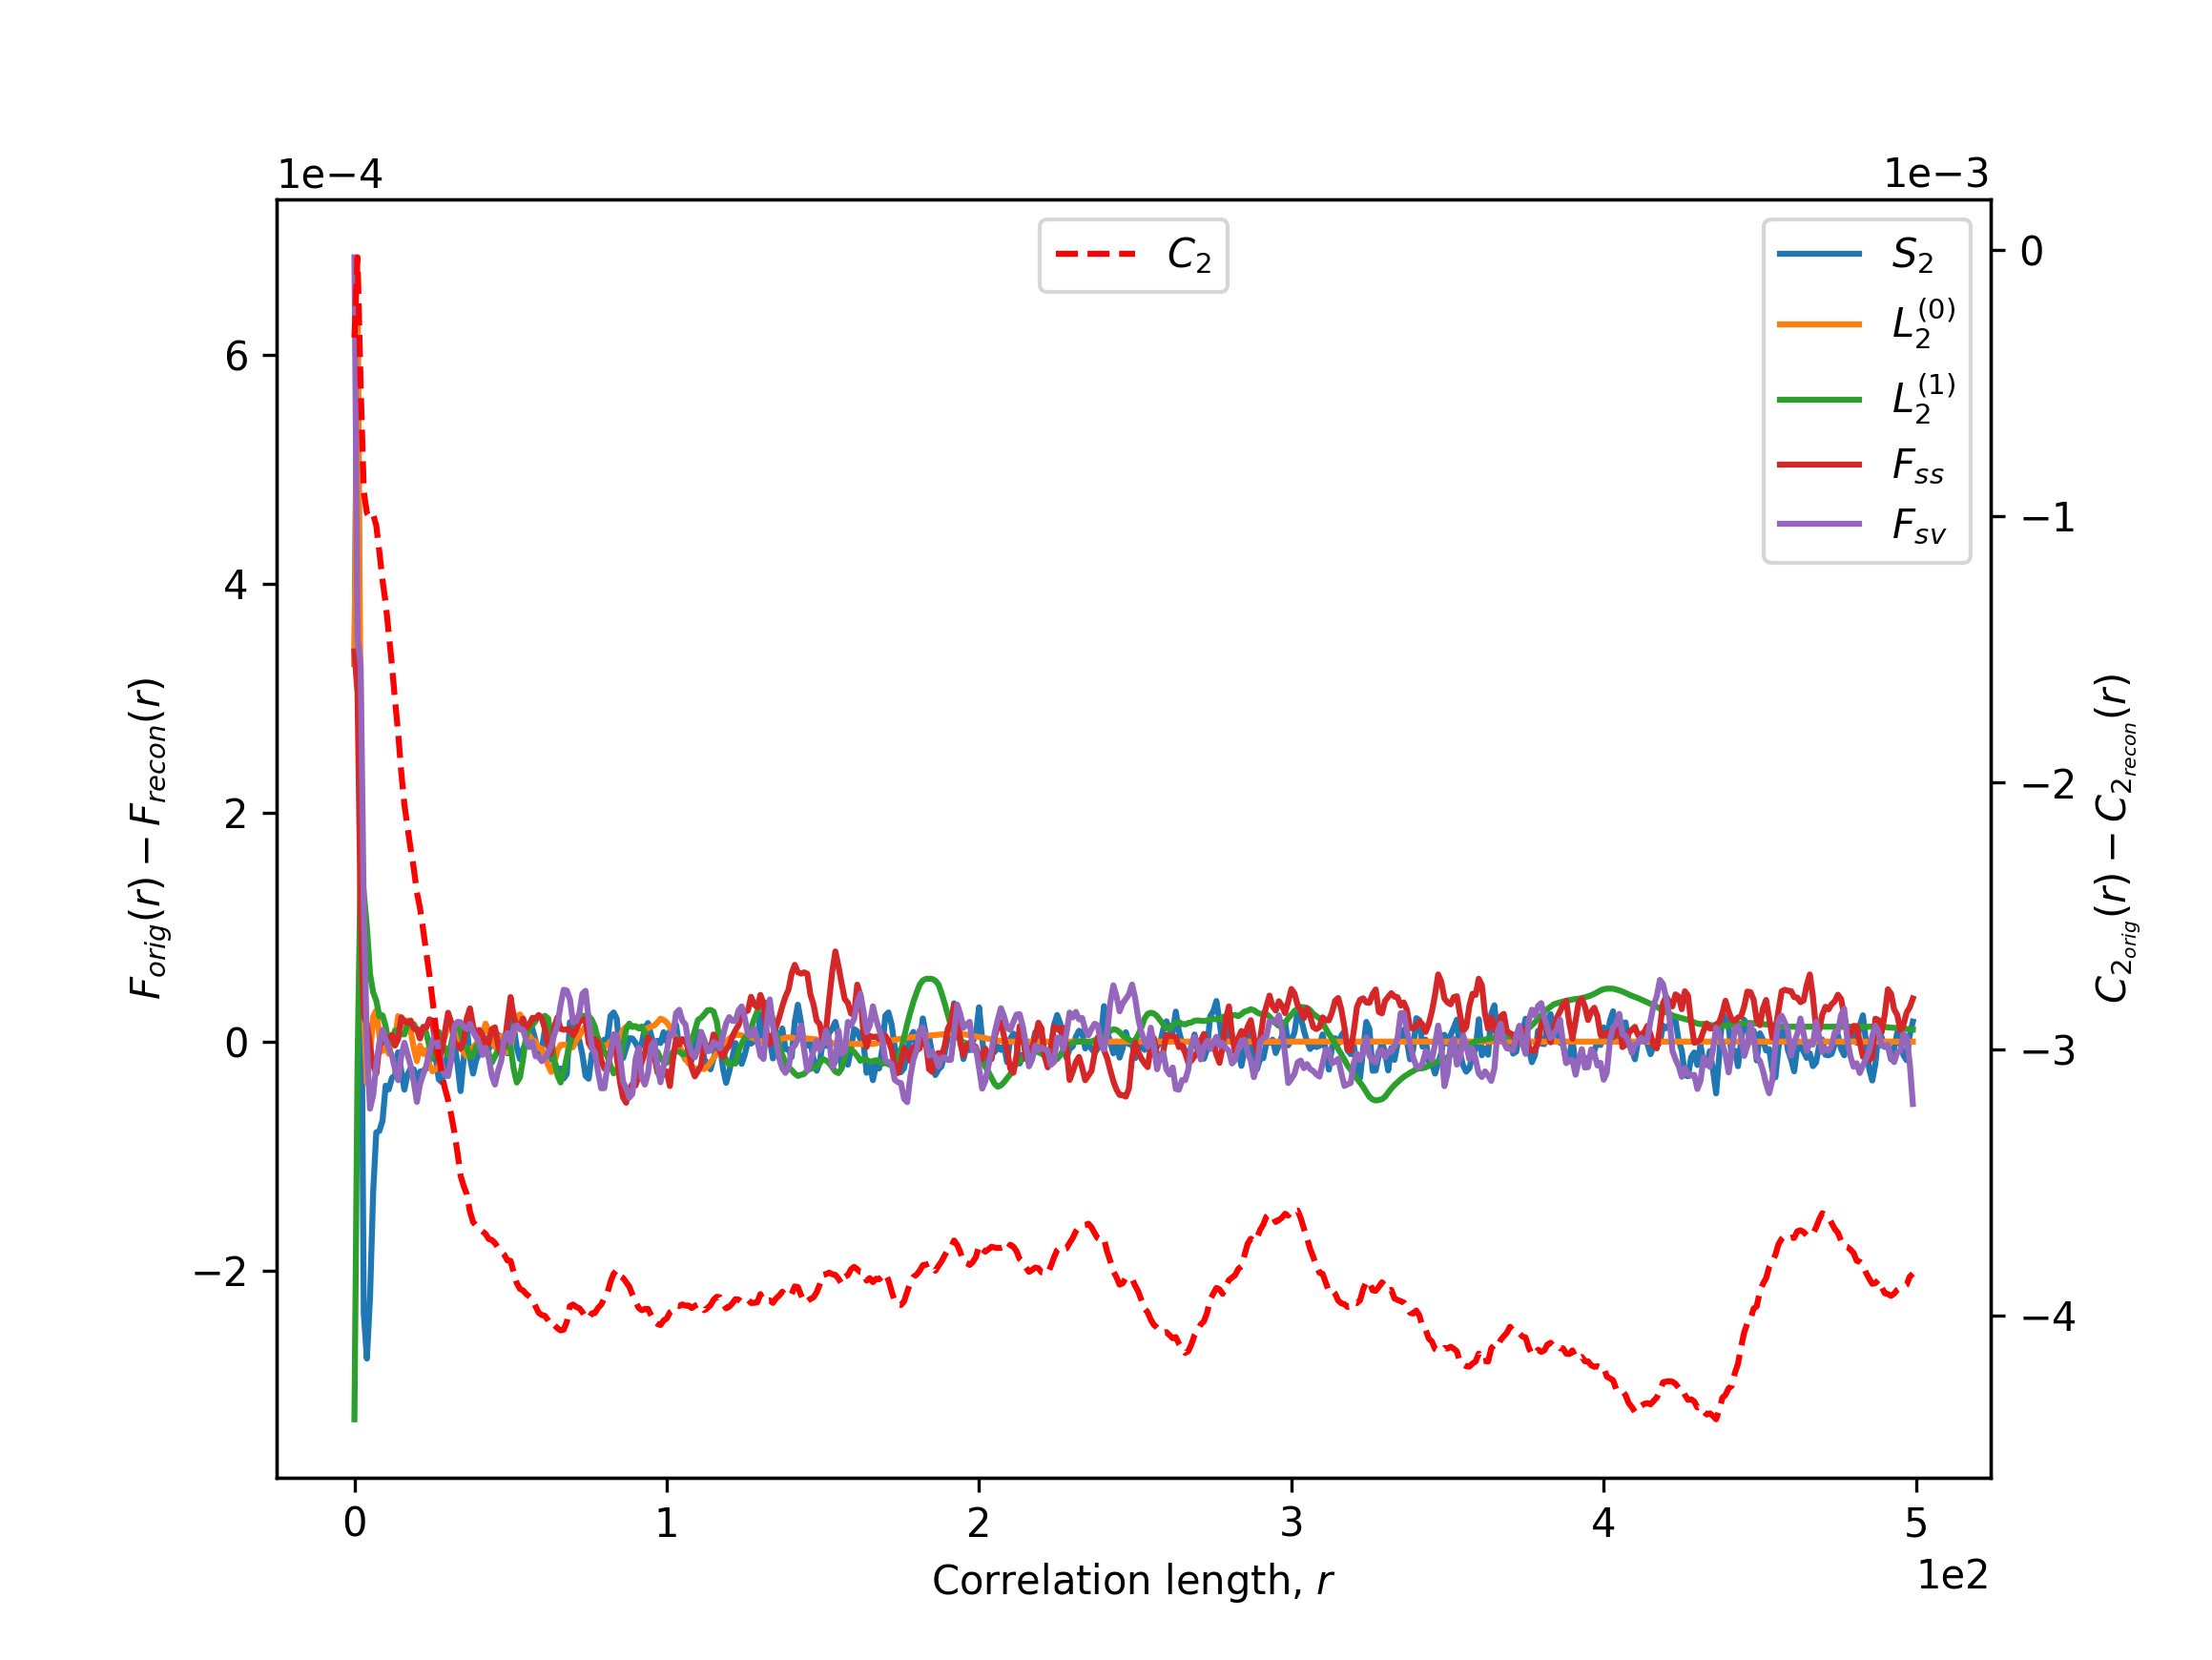
\includegraphics[width=0.3\textwidth]{../corrfns-plots/noise-all.png}
    \label{fig:noise-corr-all}}
  \vskip\baselineskip
  \subfigure[]{
    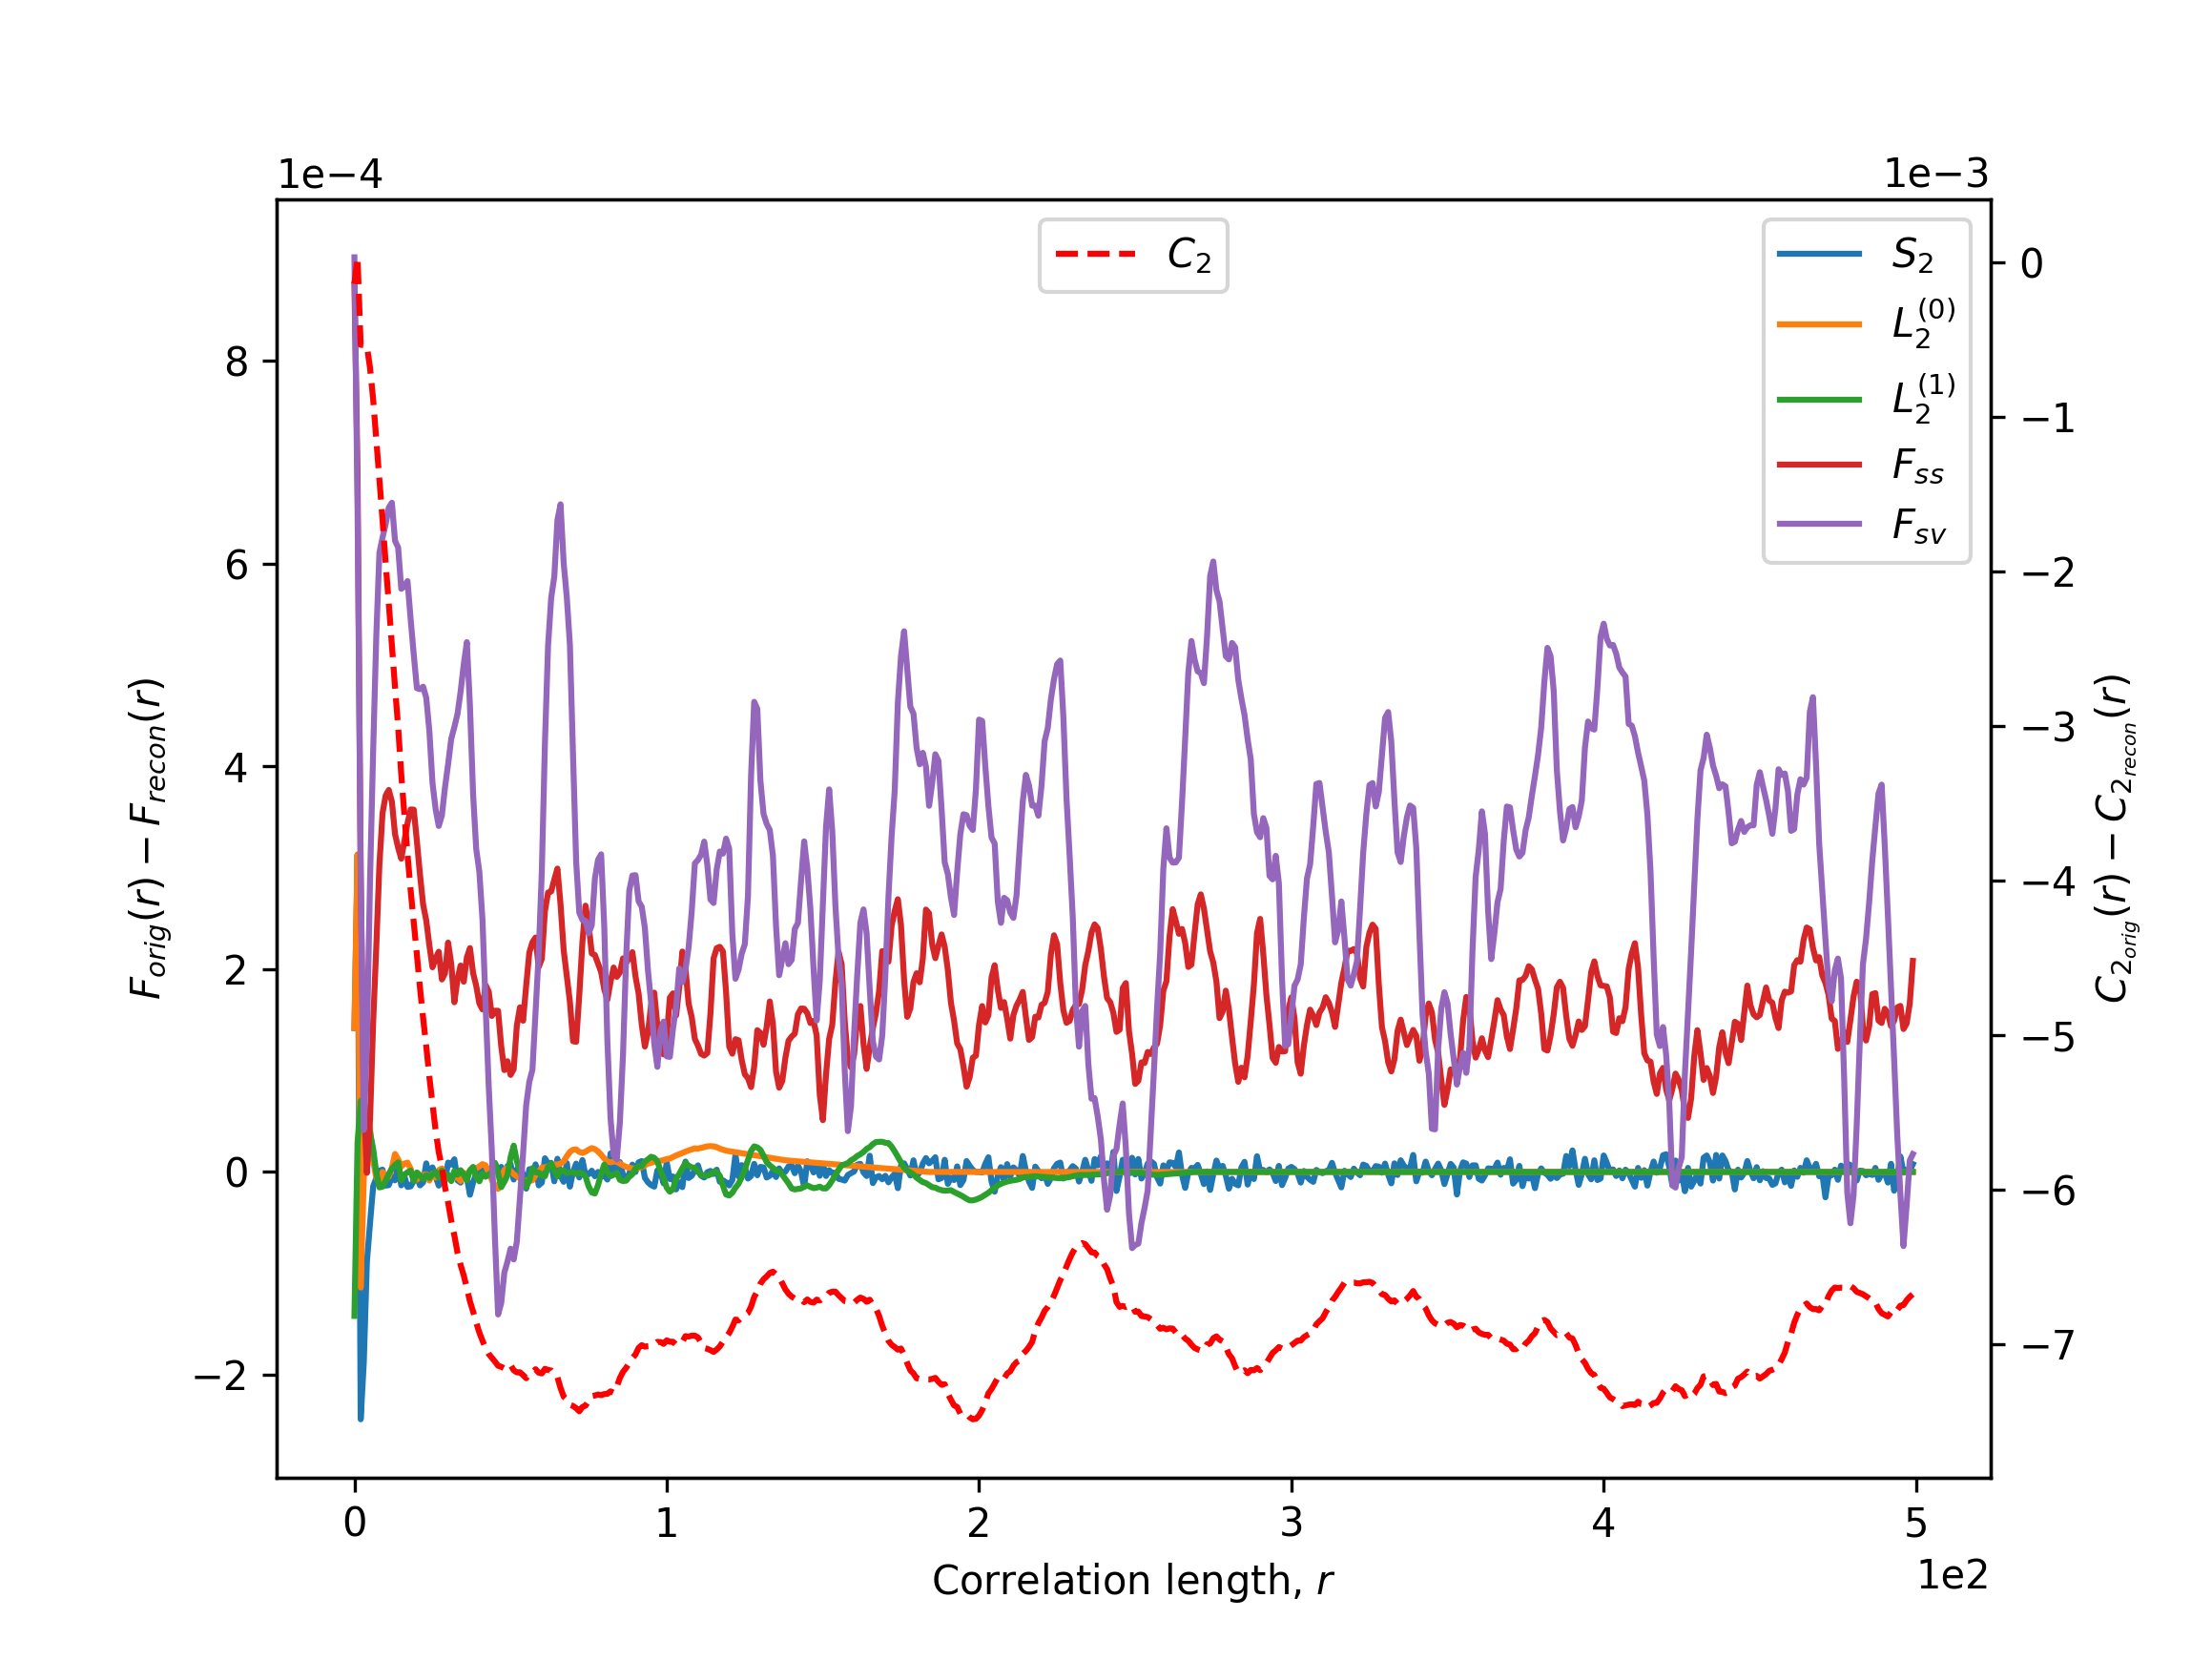
\includegraphics[width=0.3\textwidth]{../corrfns-plots/sandstone-s2l2.png}
    \label{fig:sandstone-corr-s2l2}}
  \hfill
  \subfigure[]{
    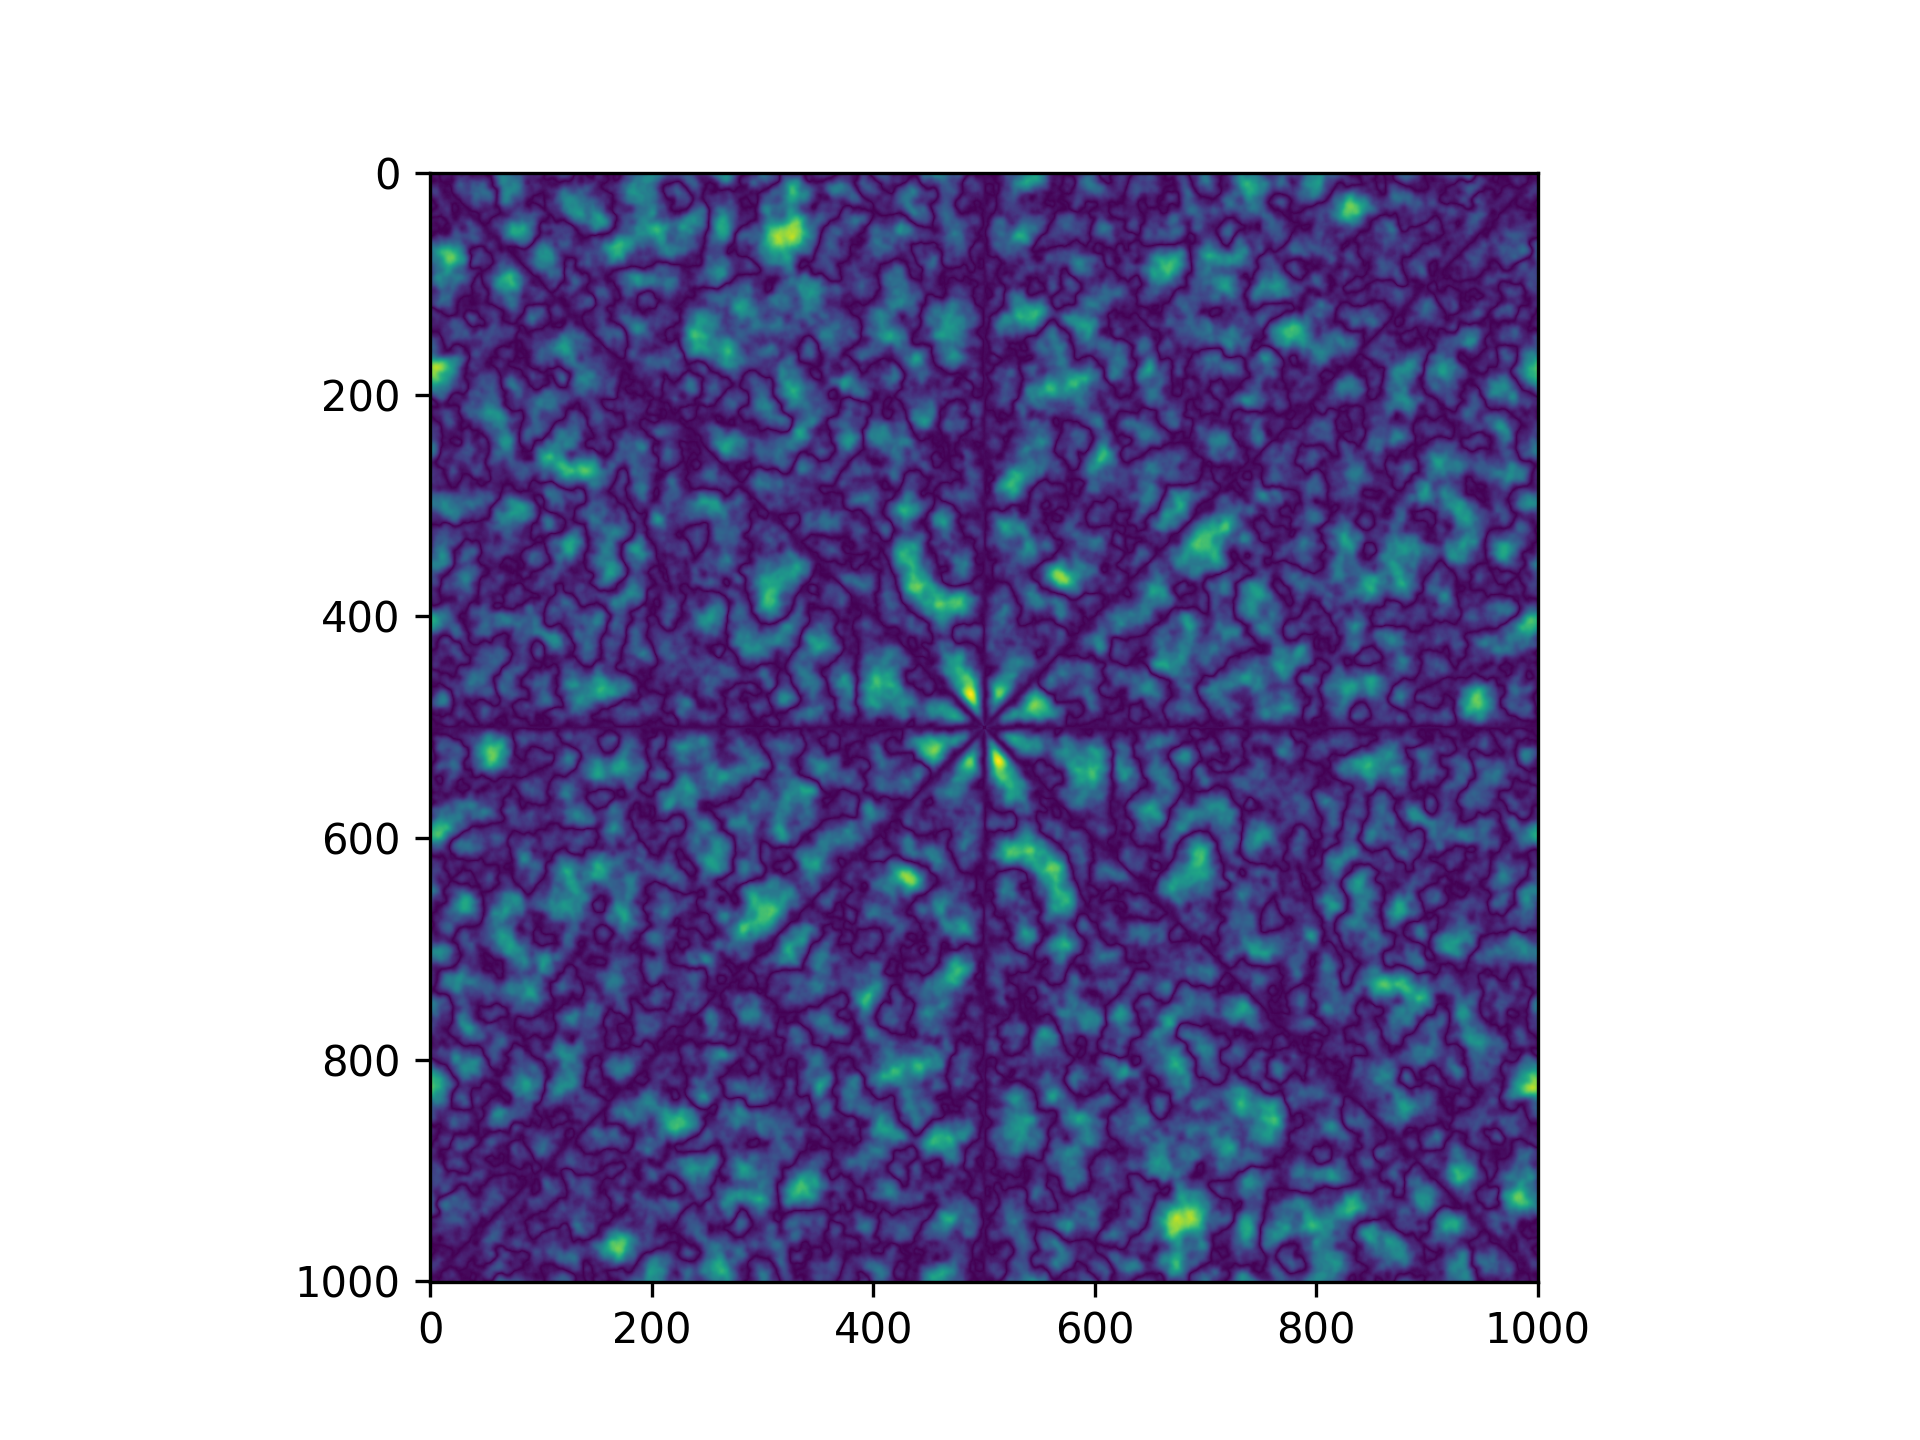
\includegraphics[width=0.3\textwidth]{../corrfns-plots/sandstone-s2l2-map.png}
    \label{fig:sandstone-corr-map}}
  \hfill
  \subfigure[]{
    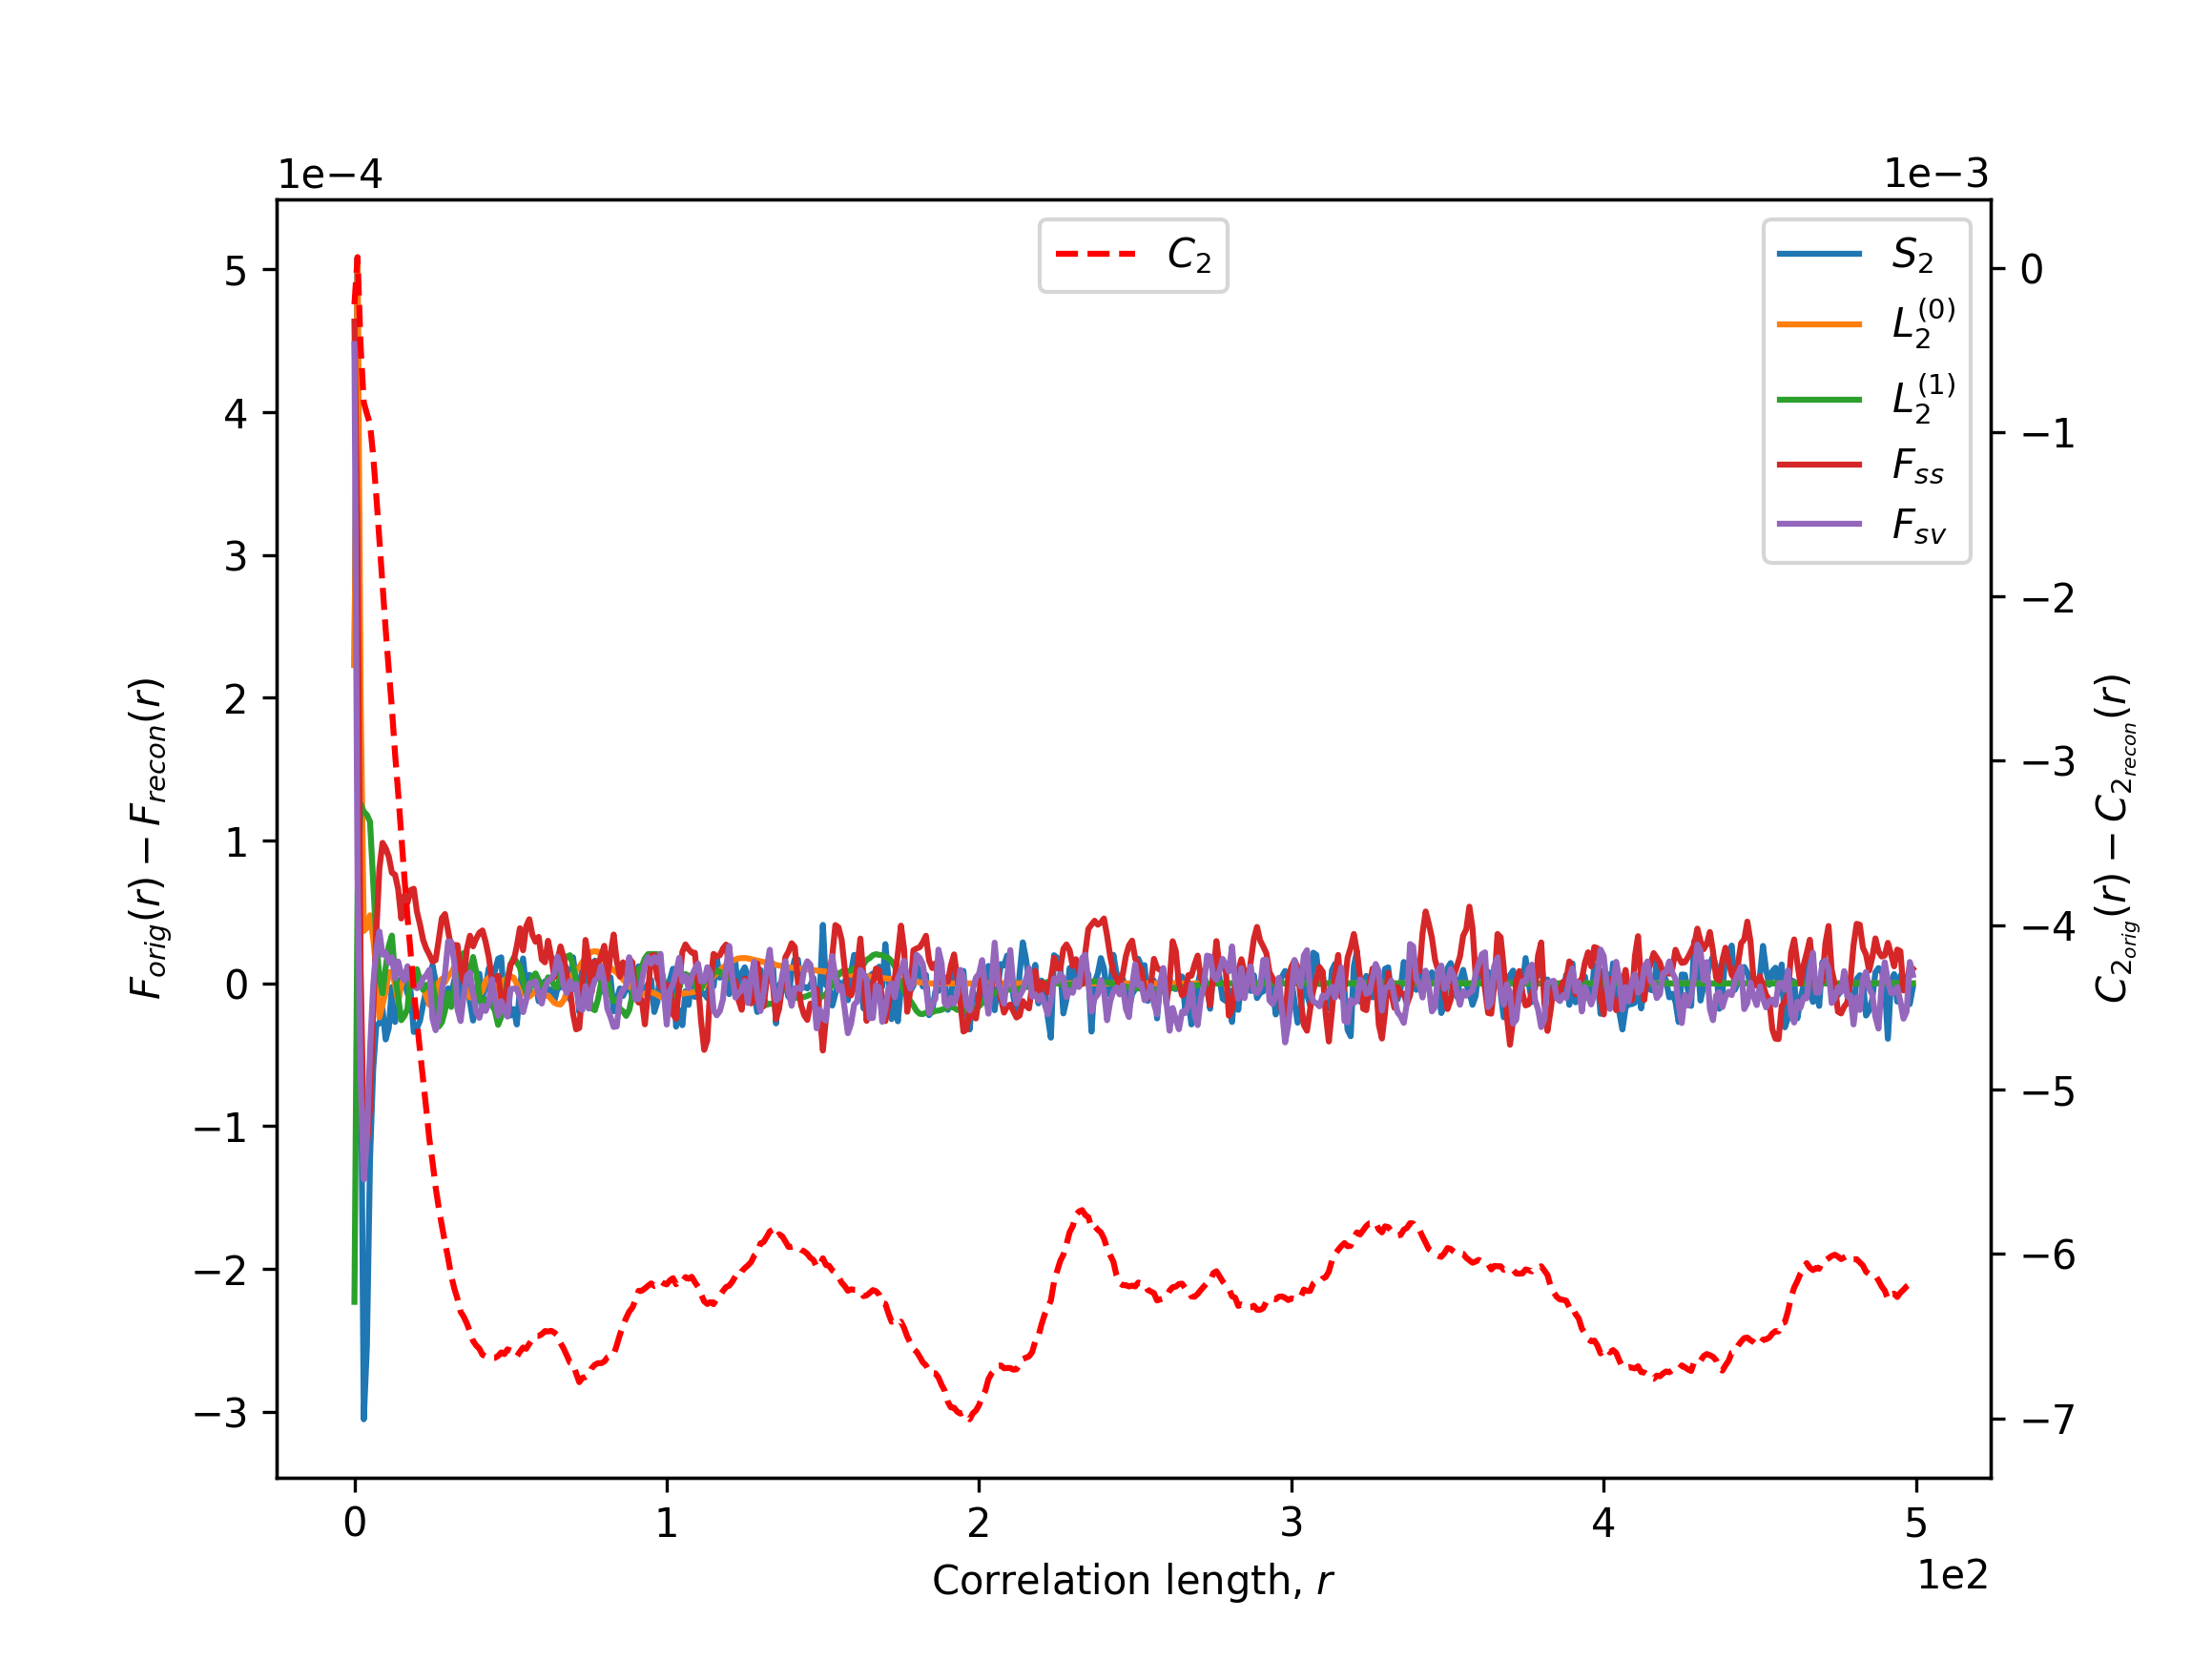
\includegraphics[width=0.3\textwidth]{../corrfns-plots/sandstone-all.png}
    \label{fig:sandstone-corr-all}}
  \caption[]{Difference between correlation functions of the original and
    reconstructed images (continued). From \cref{fig:noise-corr-s2l2} to
    \cref{fig:noise-corr-all} — value noise, from \cref{fig:sandstone-corr-s2l2}
    to \cref{fig:sandstone-corr-all} — sandstone. Images to the left are
    for reconstructions using correlation functions from the first set, images
    to the right are for reconstructions using functions from the second
    set. Images in the center are differences between two-point correlation maps
    of the original and reconstructed images.}
  \label{fig:corrfn-diff2}
\end{figure*}


\onecolumngrid
\bibliography{biblio}
\bibliographystyle{plain}

\end{document}
